\chapter{Ergebnisse}
In diesem Kapitel werden die Ergebnisse vorgestellt, die mithilfe der Implementierungen von L-Systemen und dem Space-Colonization Algorithmus produziert wurden. Es bietet sich an in vielen Fällen biologisch motivierte Begriffe zu verwenden -- beispielsweise Kanten als Äste oder Zweige zu bezeichnen -- um eine Verbindung zwischen visueller Repräsentation und graphentheoretischem Hintergrund zu schaffen.

\section{L-System-Actor}
L-Systeme ermöglichen es mithilfe bestimmter Produktionsregeln realitätsnahe Baumstrukturen zu generieren. Im Folgenden werden verschiedene natürliche Wachstumsarten mithilfe der L-System Implementierung nachgeahmt und visualisiert.
\subsection{Monopodiales Wachstum}
Ein biologischer Baum mit monopodialem Wachstumsverhalten bildet einen Hauptstamm, der stets weiterwächst, mit davon abzweigenden Nebenästen. \cite[S.14]{Deussen:05} Ein Beispiel für ein solches Wachstum ist das folgende L-System:

\begin{equation}
\begin{array}{llll}
\omega & : F(s)A(100) \\
p_1 & : A(l) &\rightarrow& F(l)\text{ }[\&(a1)\text{ }B(l)]\text{ }/(d1)\text{ }A(l*r1) \\
p_2 &  : B(l) &\rightarrow& F(l)\text{ }[-(a2)\text{ }B(l*r2)]\text{ }/(d2)\text{ }B(l*r2)
\end{array}
\label{eq:ProdMonopodial}
\end{equation} 
\cite[S.56]{ABOP:04}

Die Produktionsregel $p_1$ produziert den Hauptstamm, welcher in jeder Ableitung verlängert wird und einen Nebenast produziert, der anhand von $p_2$ ebenfalls entlang einer Hauptachse weiterwächst und weitere Nebenäste produziert. $a_1$ und $a_2$ entsprechen den Abzweigungswinkeln neuer Äste von der Hauptachse, während die Winkel $d_1$ und $d_2$ die Rotation um die Hauptachse beschreiben, bevor ein neuer Nebenast produziert wird. $r_1$ und $r_2$ entsprechen Faktoren, welche das Wachstum eines Astes pro Ableitung verkürzen, falls diese Werten unter $1$ entsprechen, und verlängern, falls Werte über $1$ vorliegen. Die Variable $s$ beschreibt die Länge des Stammes bevor das Wachstum beginnt. \cite[S.57]{ABOP:04}

Abbildung \ref{fig:LS_Monopodial} zeigt Beispiele für monopodiale Baumstrukturen, Tabelle \ref{tab:LS_Monopodial} die verwendeten Konstantenwerte. Es findet kein Einfluss durch Tropismus statt.
\begin{center}
	\begin{tabulary}{\textwidth}{|C|C|C|C|C|C|C|C|C|}
		\hline 
		Abbildung & $n$ & $a_1$ & $a_2$ & $r_1$ & $r_2$ & $d_1$ & $d_2$ & $s$ \\ 
		\hline 
		5.1a & 11 & 45.0 & 35.0 & 1.05 & 0.9 & 137.5 & 70.0 & 100.0 \\ 
		\hline 
		5.1b & 11 & 60.0 & 20.0 & 1.05 & 0.9 & 137.5 & 70.0 & 100.0 \\ 
		\hline 
		5.1c & 11 & 45.0 & 35.0 & 0.95 & 0.9 & 137.5 & 70.0 & 350.0 \\ 
		\hline 
		5.1d & 11 & 77.0 & -37.0 & 1.05 & 0.85 & 137.5 & -70.0 & 200.0 \\ 
		\hline 
	\end{tabulary} 
	\captionof{table}{Konstantenwerte der in Abbildung \ref{fig:LS_Monopodial} dargestellten monopodialen Baumstrukturen.} 
	\label{tab:LS_Monopodial}
\end{center}


\begin{figure} [hbtp]
	\centering
	\begin{subfigure}[t]{.45\textwidth}
		\centering
		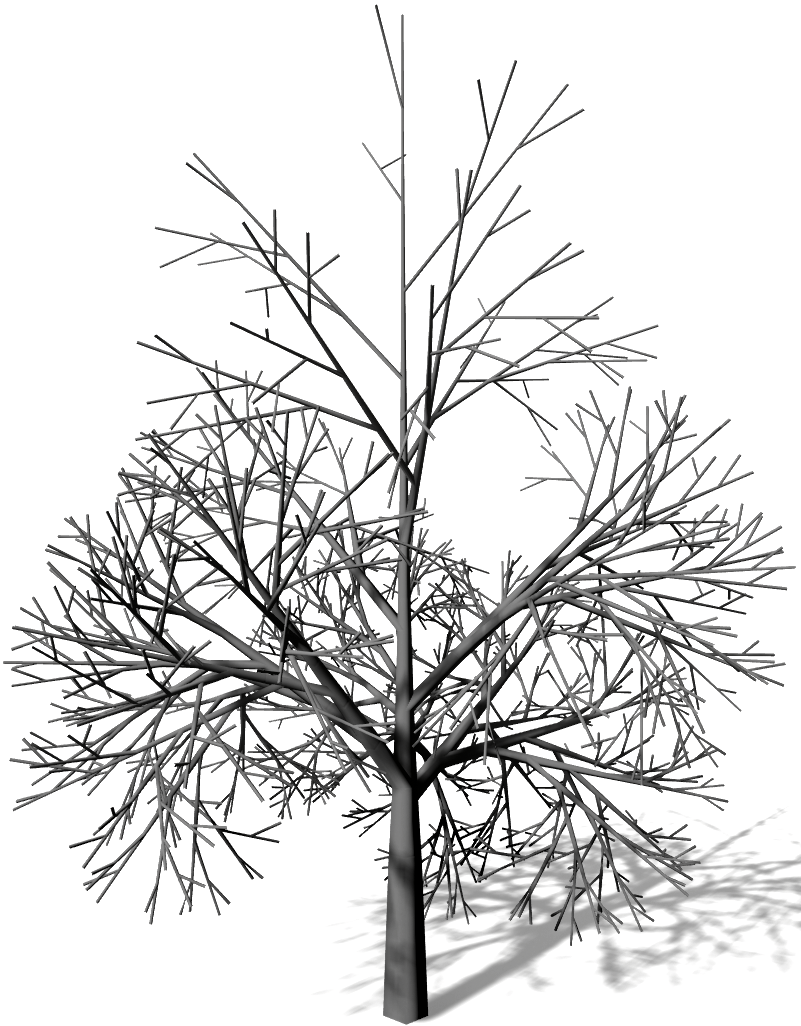
\includegraphics[height=.21\textheight]{images/LS_Monopodial_1.png}
		\caption{}
		\label{subfig:LS_Monopodial_1}
	\end{subfigure}
	\begin{subfigure}[t]{.45\textwidth}
		\centering
		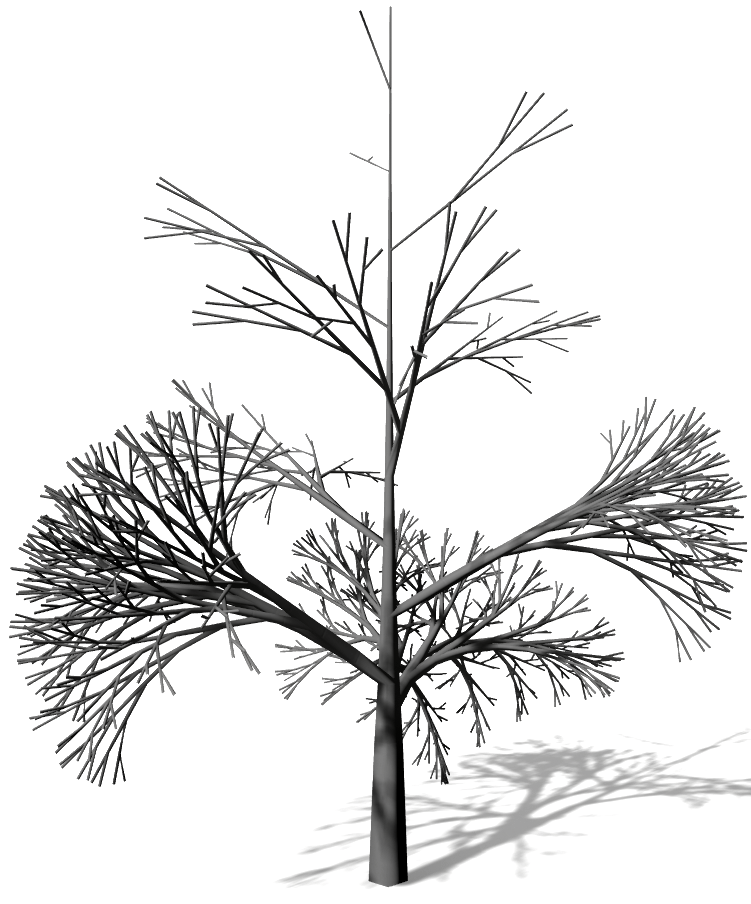
\includegraphics[height=.21\textheight]{images/LS_Monopodial_2.png}
		\caption{}
		\label{subfig:LS_Monopodial_2}
	\end{subfigure}	
	\begin{subfigure}[t]{.45\textwidth}
		\centering
		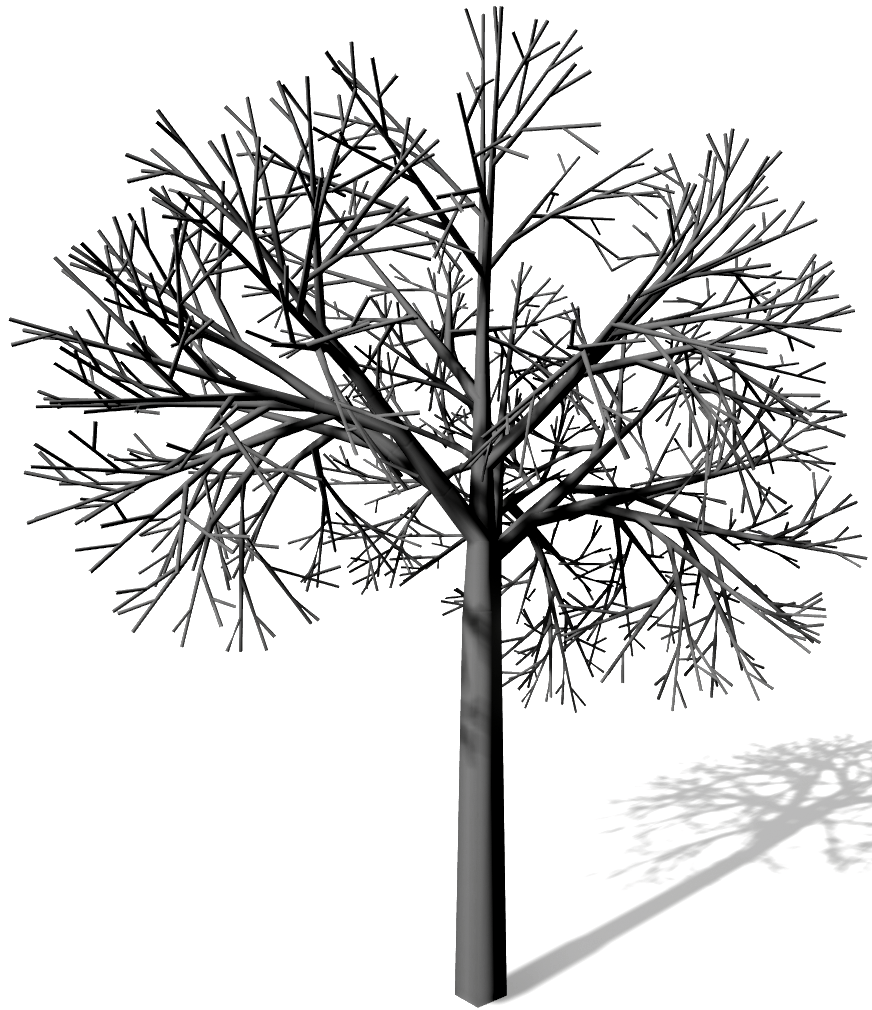
\includegraphics[height=.21\textheight]{images/LS_Monopodial_3.png}
		\caption{}
		\label{subfig:LS_Monopodial_3}
	\end{subfigure}
	\begin{subfigure}[t]{.45\textwidth}
		\centering
		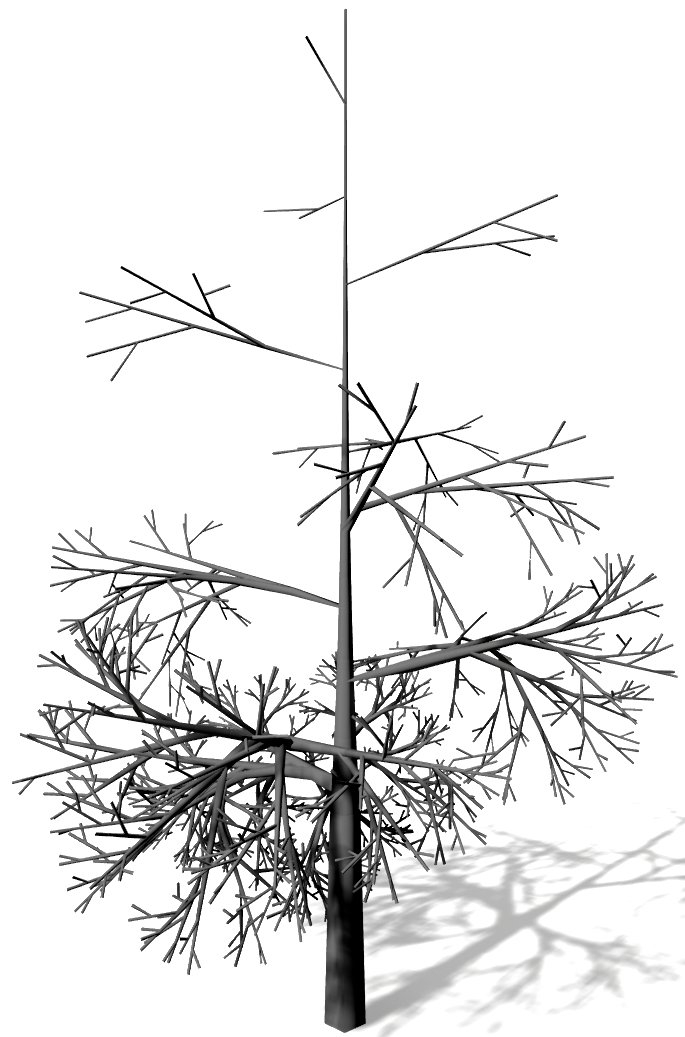
\includegraphics[height=.21\textheight]{images/LS_Monopodial_4.png}
		\caption{}
		\label{subfig:LS_Monopodial_4}
	\end{subfigure}
	\caption{Beispiele monopodialen Wachstums, entspricht der n-fachen Ableitung des Axioms anhand der Produktionsregeln aus Gleichung \ref{eq:ProdMonopodial}. Eigene Abbildungen.}
	\label{fig:LS_Monopodial}
\end{figure}

\subsection{Sympodiales Wachstum}
Beim sympodialen Wachstum bildet ein Ast mehrere Abzweigungen in einem Winkel ungleich $0\degree$. Der sich verzweigende Ast wächst daraufhin nicht weiter. \cite[S.14]{Deussen:05} \cite[S.58]{ABOP:04} Das folgende L-System simuliert ein solches Wachstum:

\begin{equation}
\begin{array}{llll}
\omega & : F(100)A(150) \\
p_1 & : A(l) &\rightarrow& F(l)\text{ }[\&(a1)\text{ }B(l*r1)]\text{ }/(180)\text{ }[\&(a2)\text{ }B(l*r2)] \\
p_2 &  : B(l) &\rightarrow& F(l)\text{ }[+(a1)\text{ }/(d1)\text{ }B(l*r1)]\text{ }[-(a2)\text{ }\backslash(d2)\text{ }B(l*r2)]
\end{array}
\label{eq:ProdSympodial}
\end{equation} 

\cite[S.59]{ABOP:04}

Die Produktionsregel $p_1$ beschreibt die Bildung der ersten, sich gegenüberliegenden, Abzweigungen während $p_2$ das Wachstum der abzweigenden Äste beschreibt, welche sich ebenfalls zu zwei Nebenästen aufteilen. $a_1$ und $a_2$ entsprechen den Abzweigungswinkeln, $r_1$ und $r_2$ den Wachstumsfaktoren pro Ableitung der Nebenäste. $d_1$ und $d_2$ beschreiben die Rotation eines Nebenastes um seine eigene Achse, bevor die nächste Abzweigung entsteht.

Abbildung \ref{fig:LS_Sympodial} zeigt Beispiele für sympodiale Baumstrukturen, Tabelle \ref{tab:LS_Sympodial} die verwendeten Konstantenwerte. Es findet kein Einfluss durch Tropismus statt.

\begin{center}
	\begin{tabulary}{\textwidth}{|C|C|C|C|C|C|C|C|}
		\hline 
		Abbildung & $n$ & $a_1$ & $a_2$ & $r_1$ & $r_2$ & $d_1$ & $d_2$ \\ 
		\hline 
		5.2a & 10 & 5.0 & 65.0 & 0.9 & 0.75 & 50.0 & 50.0 \\ 
		\hline 
		5.2b & 10 & 20.0 & 50.0 & 0.9 & 0.75 & 50.0 & 50.0 \\ 
		\hline 
		5.2c & 10 & 35.0 & 35.0 & 1.0 & 0.8 & 50.0 & 50.0 \\ 
		\hline 
		5.2d & 10 & 30.0 & 40.0 & 0.95 & 0.9 & 110.0 & 110.0 \\ 
		\hline 
	\end{tabulary} 
	\captionof{table}{Konstantenwerte der in Abbildung \ref{fig:LS_Sympodial} dargestellten sympodialen Baumstrukturen.} 
	\label{tab:LS_Sympodial}
\end{center}

\begin{figure} [hbtp]
	\centering
	\begin{subfigure}[t]{.45\textwidth}
		\centering
		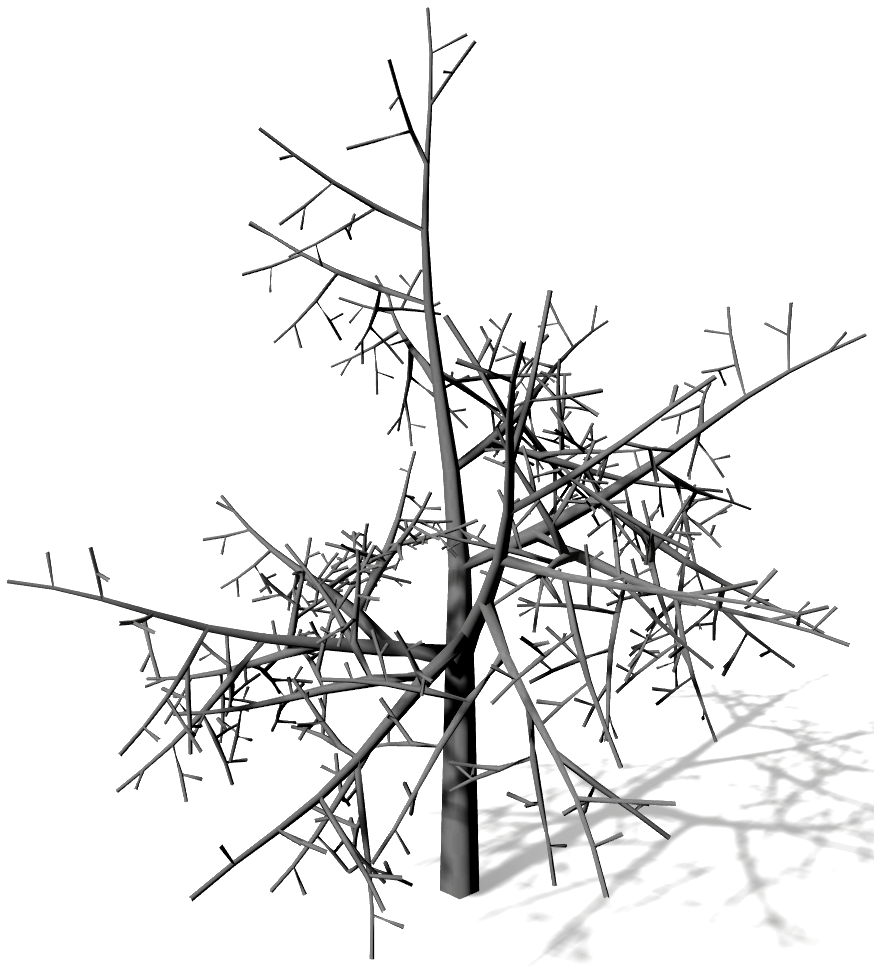
\includegraphics[height=.21\textheight]{images/LS_Sympodial_1.png}
		\caption{}
		\label{subfig:LS_Sympodial_1}
	\end{subfigure}
	\begin{subfigure}[t]{.45\textwidth}
		\centering
		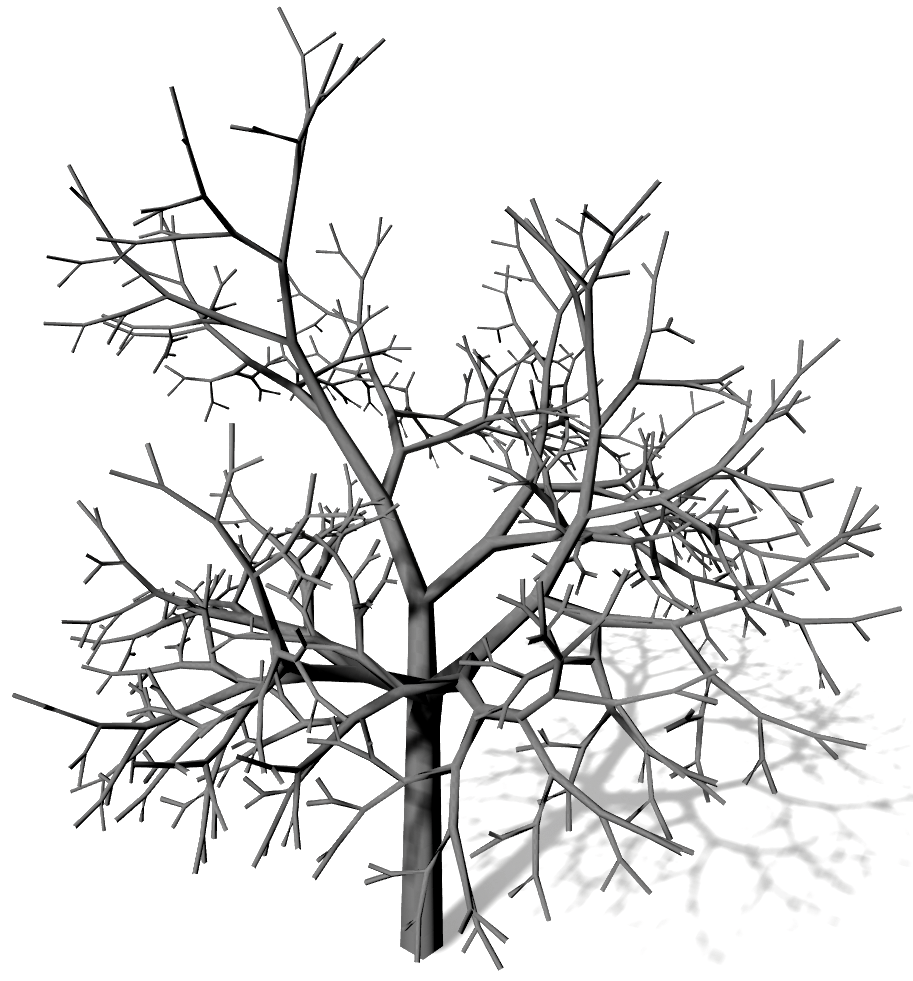
\includegraphics[height=.21\textheight]{images/LS_Sympodial_2.png}
		\caption{}
		\label{subfig:LS_Sympodial_2}
	\end{subfigure}	
	\begin{subfigure}[t]{.45\textwidth}
		\centering
		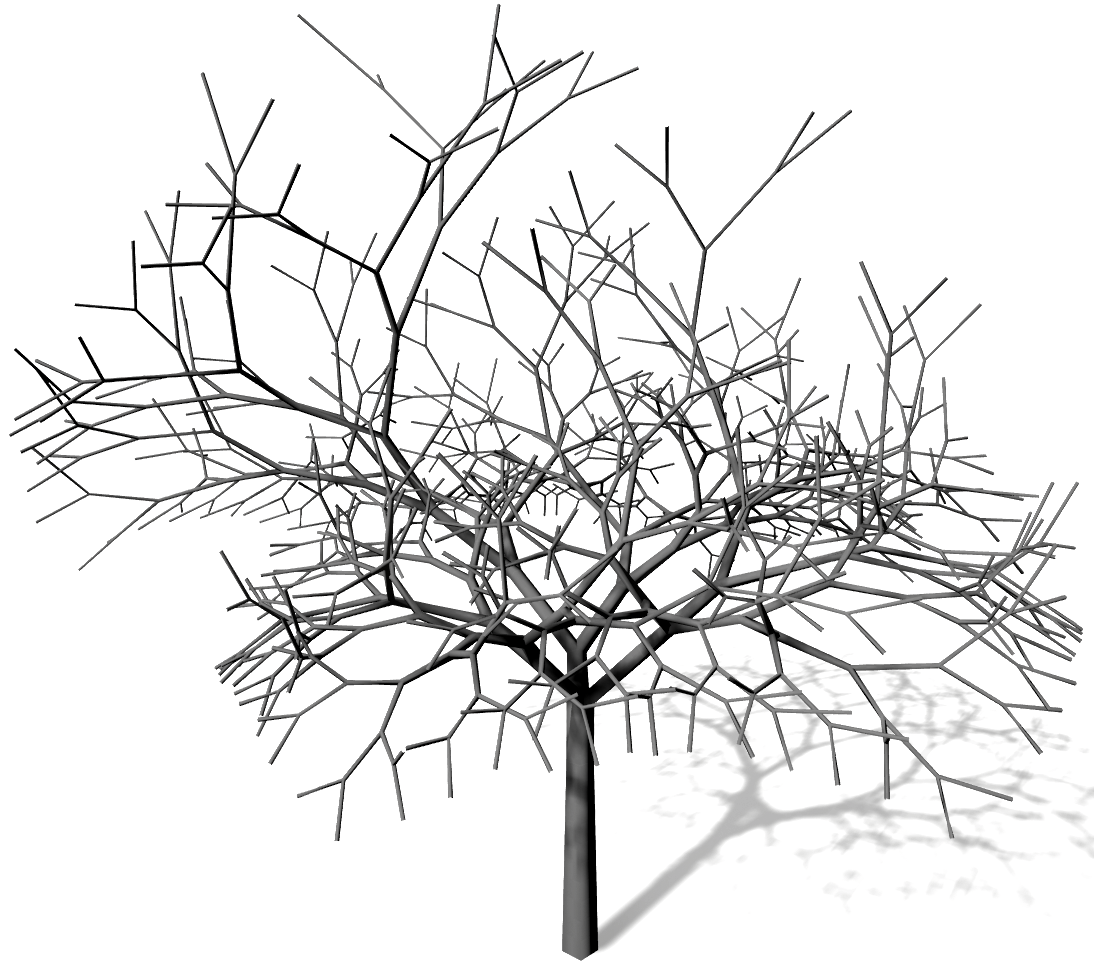
\includegraphics[height=.21\textheight]{images/LS_Sympodial_3.png}
		\caption{}
		\label{subfig:LS_Sympodial_3}
	\end{subfigure}
	\begin{subfigure}[t]{.45\textwidth}
		\centering
		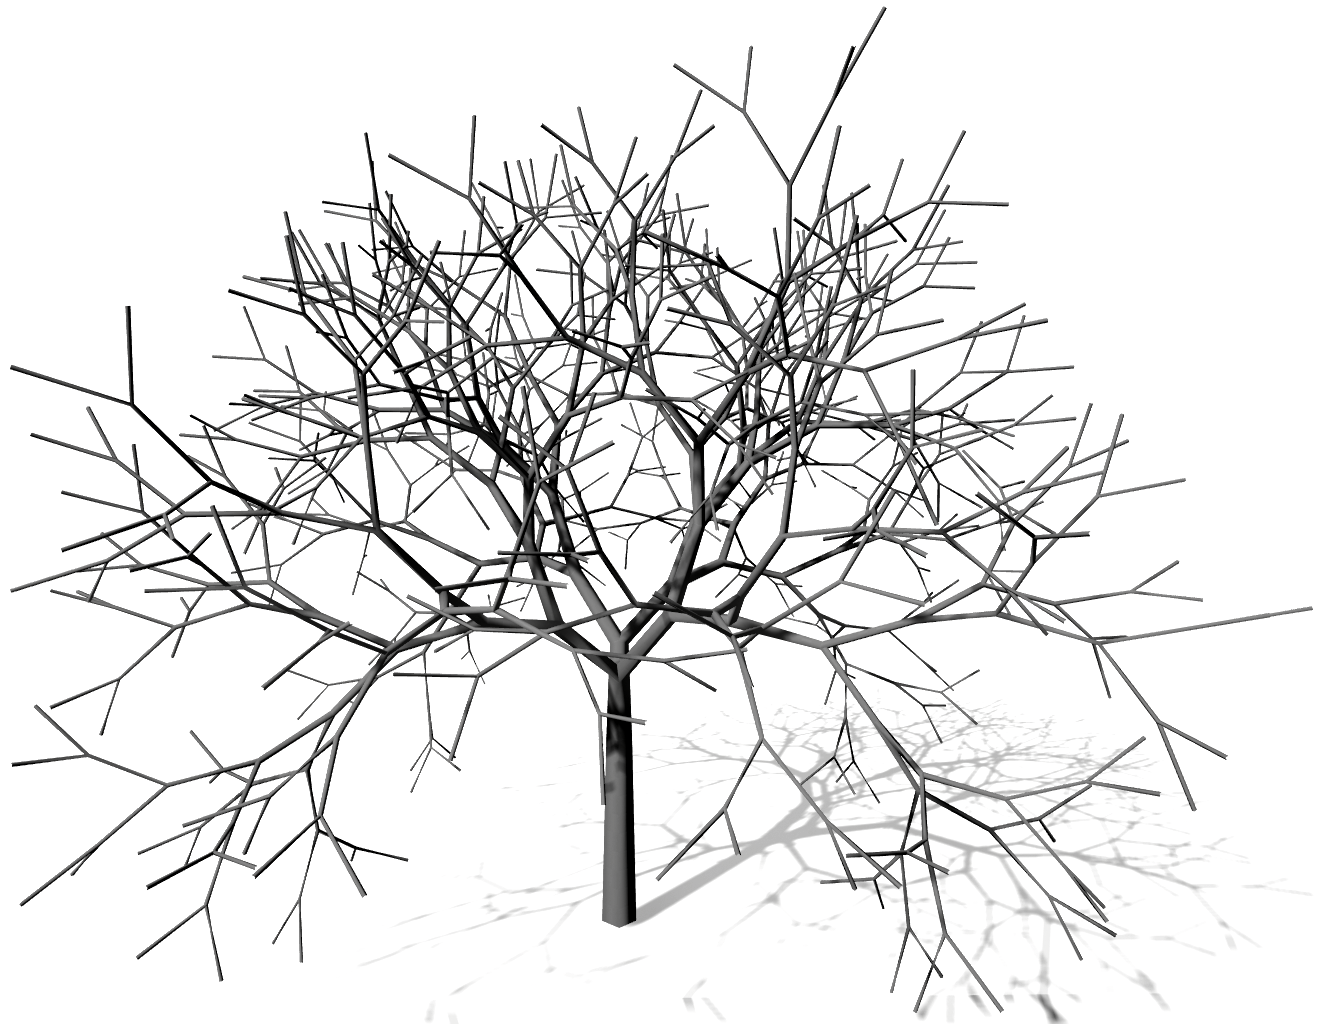
\includegraphics[height=.21\textheight]{images/LS_Sympodial_4.png}
		\caption{}
		\label{subfig:LS_Sympodial_4}
	\end{subfigure}
	\caption{Beispiele sympodialen Wachstums, entspricht der n-fachen Ableitung des Axioms anhand der Produktionsregeln aus Gleichung \ref{eq:ProdSympodial}. Eigene Abbildungen.}
	\label{fig:LS_Sympodial}
\end{figure}


\subsection{Ternäre Verzweigungen}

Eine andere Herangehensweise zur Bestimmung von L-Systemen für realistisch wirkende Baumstrukturen ist die Beschreibung von Selbstähnlichkeit, wie sie oft in der Natur zu finden ist. \cite[S.173]{ABOP:04} Das L-System aus Gleichung \ref{eq:ProdTernary} entspricht einem Wachstum, in welchem drei Abzweigungen mithilfe von Produktion $p_1$ auf dieselbe Art erstellt werden. In Produktion $p_2$ wird beschrieben wie Kanten aus vorhergehenden Ableitungen um einen Faktor $l_r$ verlängert werden. \cite[S.58]{ABOP:04}

\begin{equation}
\begin{array}{llll}
\omega & : /(45)A \\
p_1 & : A &\rightarrow& F(l_s)\text{ }[\&(a)\text{ }F(l_s)\text{ }A]\text{ }/(d1)\text{ }[\&(a)\text{ }F(l_s)\text{ }A]\text{ }/(d2)\text{ }[\&(a)\text{ }F(l_s)\text{ }A] \\
p_2 &  : F(l) &\rightarrow& F(l * l_r)
\end{array}
\label{eq:ProdTernary}
\end{equation} 
\cite[S.60]{ABOP:04}

$a$ entspricht dem Abzweigungswinkel von der Ursprungsachse, $d_1$ und $d_2$ der Rotation um die Achse, bevor eine neue Abzweigung produziert wird. $l_s$ ist die Anfangslänge der Kanten. \cite[S.58]{ABOP:04}

Abbildung \ref{fig:LS_Ternary} zeigt verschiedene ternär verzweigte Baumstrukturen, die auf den in Tabelle \ref{tab:LS_Ternary} gelisteten Konstantenwerten aufgebaut sind.

\begin{center}
	\begin{tabulary}{\textwidth}{|C|C|C|C|C|C|C|}
		\hline 
		Abbildung & $n$ & $a$ & $d_1$ & $d_2$ & $l_r$ & $l_s$ \\ 
		\hline 
		5.3a & 6 & 19.0 & 95.0 & 132.0 & 1.1 & 50.0 \\ 
		\hline 
		5.3b & 8 & 19.0 & 137.5 & 137.5 & 1.2 & 50.0 \\ 
		\hline 
		5.3c & 8 & 27.0 & 77.0 & 77.0 & 1.3 & 50.0 \\ 
		\hline 
		5.3d & 8 & 31.0 & 120.0 & 190.0 & 1.2 & 50.0 \\ 
		\hline 
	\end{tabulary} 
	\captionof{table}{Konstantenwerte der in Abbildung \ref{fig:LS_Ternary} dargestellten ternär verzweigten Baumstrukturen.} 
	\label{tab:LS_Ternary}
\end{center}

\begin{figure} [hbtp]
	\centering
	\begin{subfigure}[t]{.45\textwidth}
		\centering
		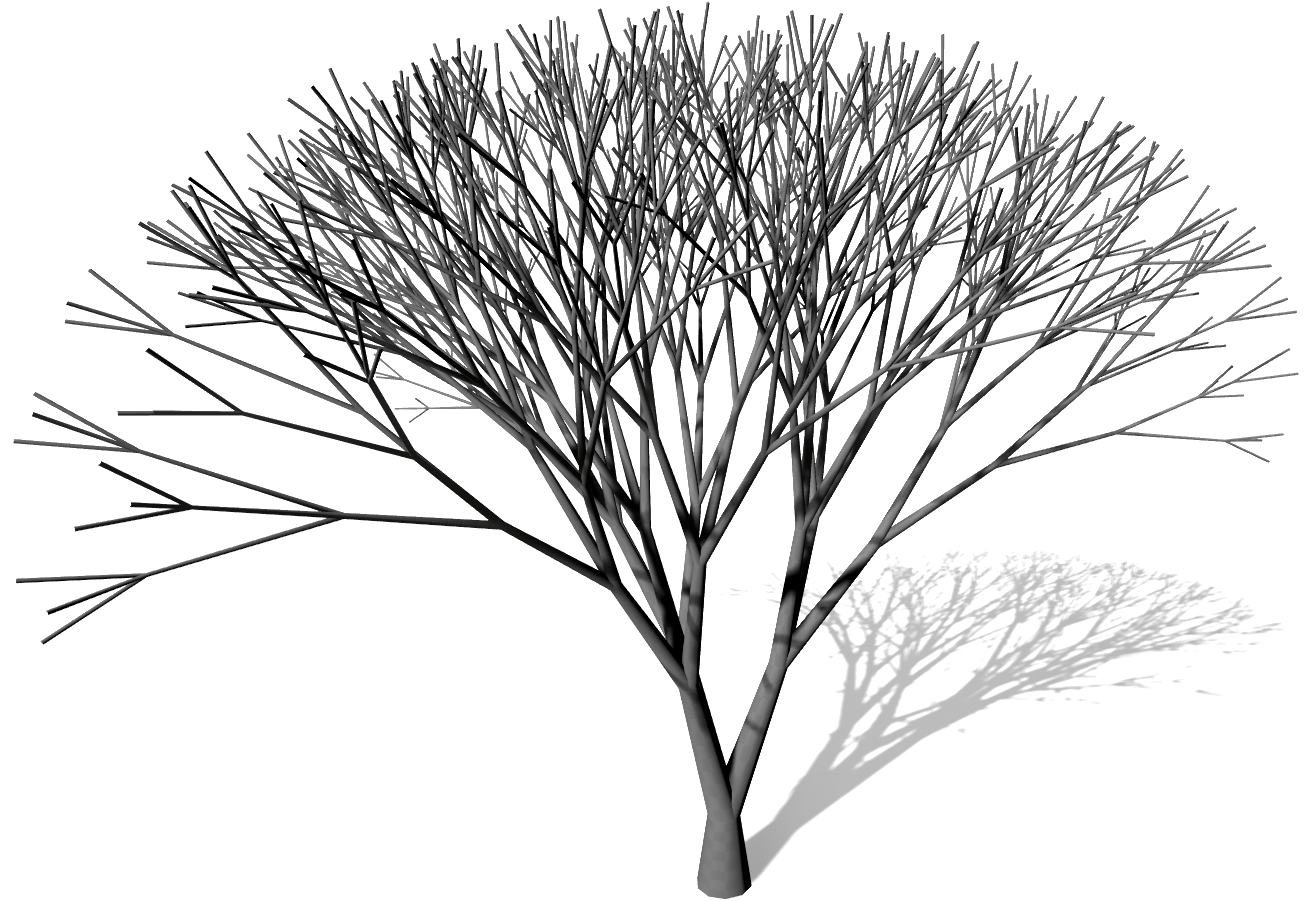
\includegraphics[width=\linewidth]{images/LS_Ternary_1.png}
		\caption{}
		\label{subfig:LS_Ternary_1}
	\end{subfigure}
	\begin{subfigure}[t]{.45\textwidth}
		\centering
		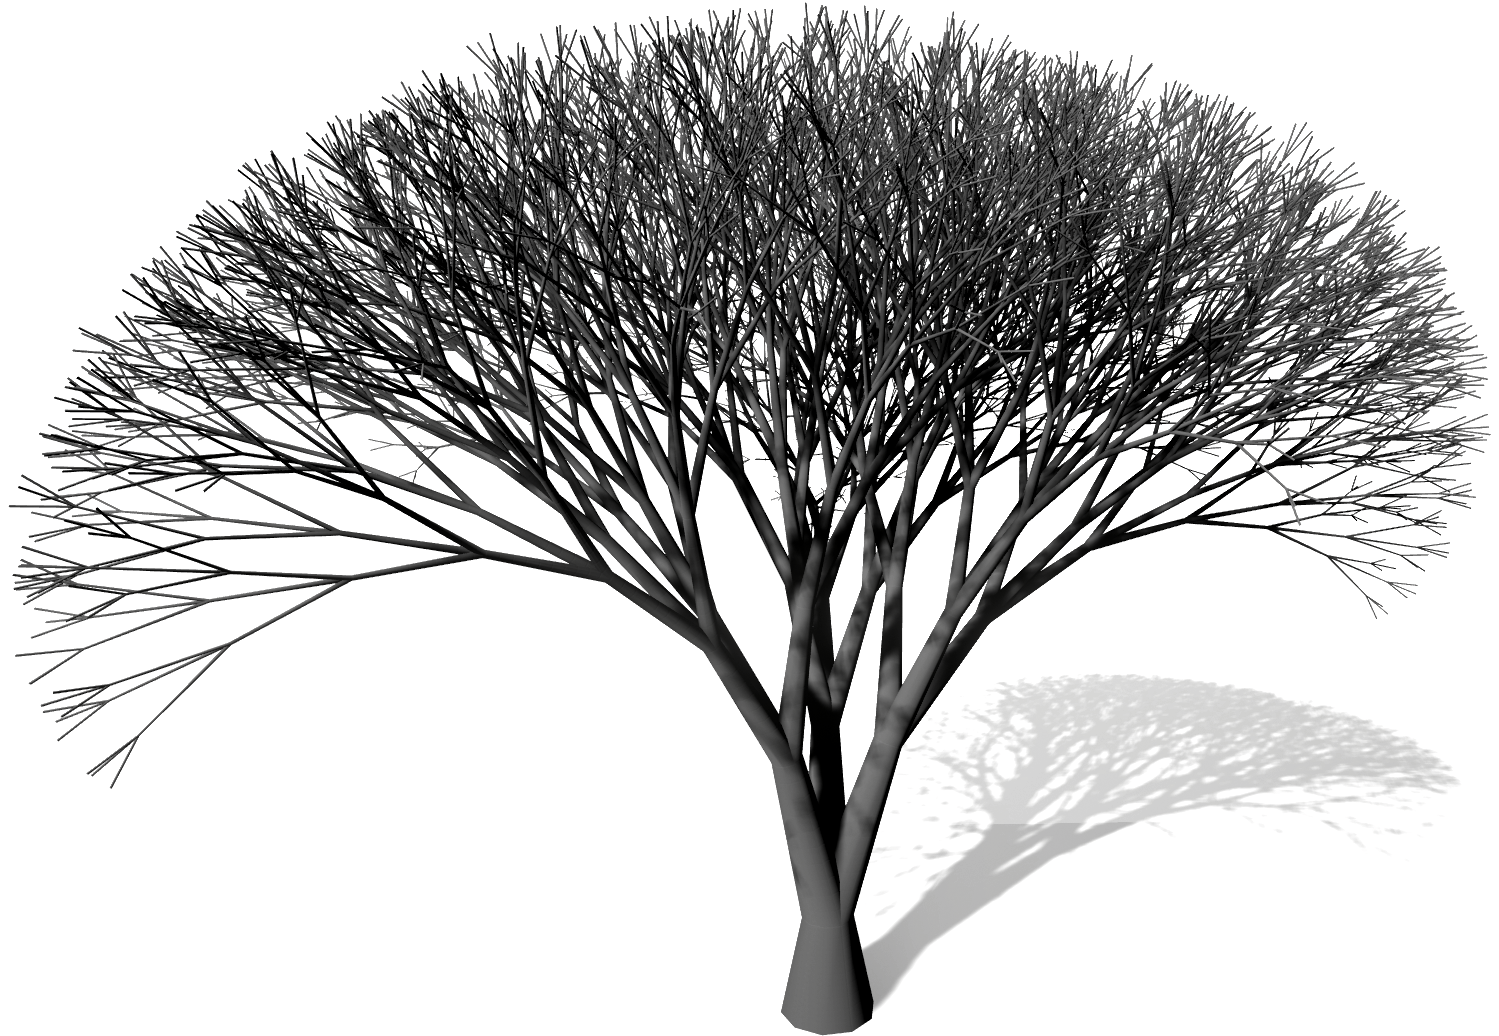
\includegraphics[width=\linewidth]{images/LS_Ternary_2.png}
		\caption{}
		\label{subfig:LS_Ternary_2}
	\end{subfigure}	
	\begin{subfigure}[t]{.45\textwidth}
		\centering
		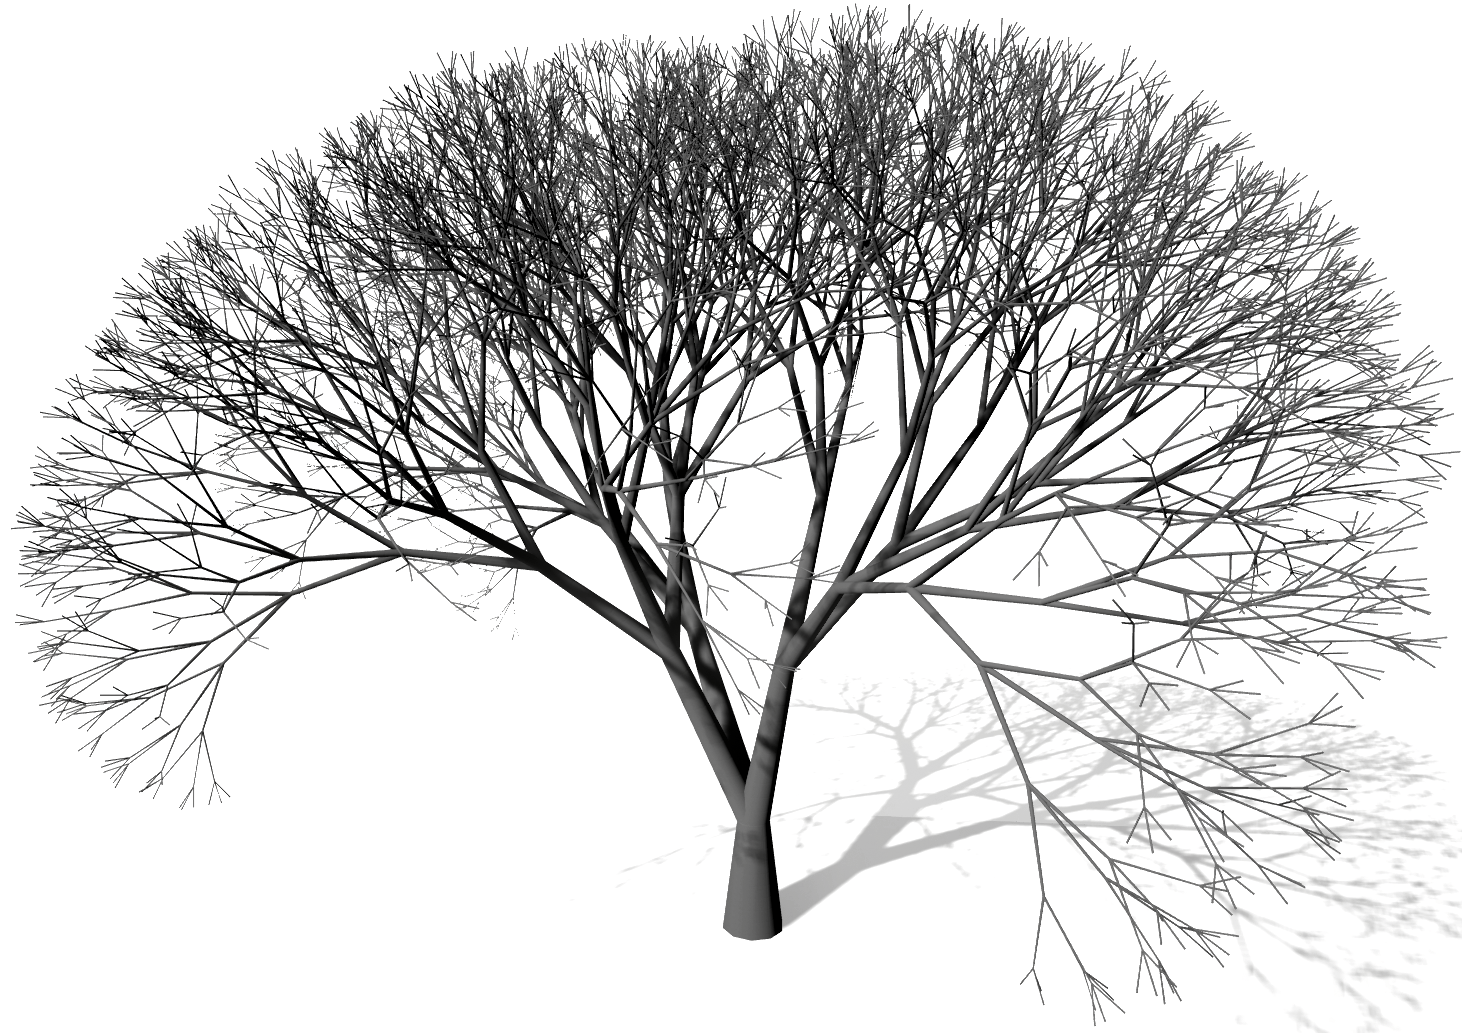
\includegraphics[width=\linewidth]{images/LS_Ternary_3.png}
		\caption{}
		\label{subfig:LS_Ternary_3}
	\end{subfigure}
	\begin{subfigure}[t]{.45\textwidth}
		\centering
		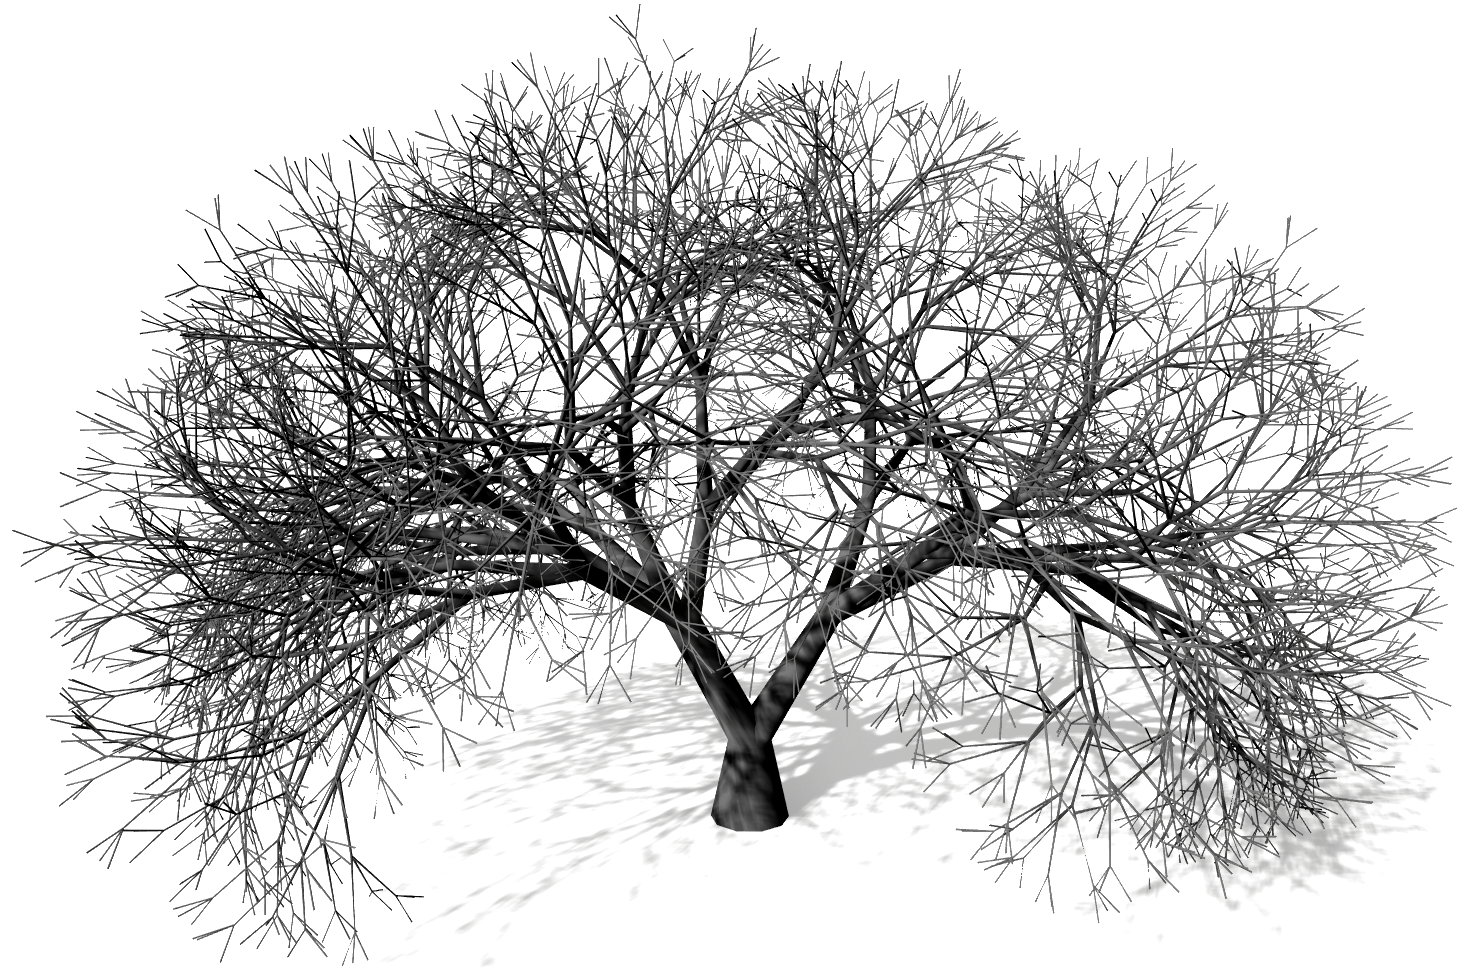
\includegraphics[width=\linewidth]{images/LS_Ternary_4.png}
		\caption{}
		\label{subfig:LS_Ternary_4}
	\end{subfigure}
	\caption{Beispiele ternären Wachstums, entspricht der n-fachen Ableitung des Axioms anhand der Produktionsregeln aus Gleichung \ref{eq:ProdTernary}. Eigene Abbildungen.}
	\label{fig:LS_Ternary}
\end{figure}


\subsection{Tropismus}

Der Einfluss von Tropismus führt, bei Eingabe derselben Werte bei den restlichen Parametern, zu visuell unterschiedlichen Ergebnissen. Dadurch können reale Einflüsse wie die Einwirkung von Wind, Sonne und Gravitation simuliert sowie die Wiederverwendbarkeit von L-System Definitionen erhöht werden. \cite[S.58]{ABOP:04}

Abbildung \ref{fig:LS_Ternary_Tropism} zeigt den Einfluss von Tropismus auf Baumstrukturen aus Abbildung \ref{fig:LS_Ternary}, welche ohne die Einwirkung von Tropismus produziert wurden.


\begin{figure} [hbtp]
	\centering
	\begin{subfigure}[t]{.45\textwidth}
		\centering
		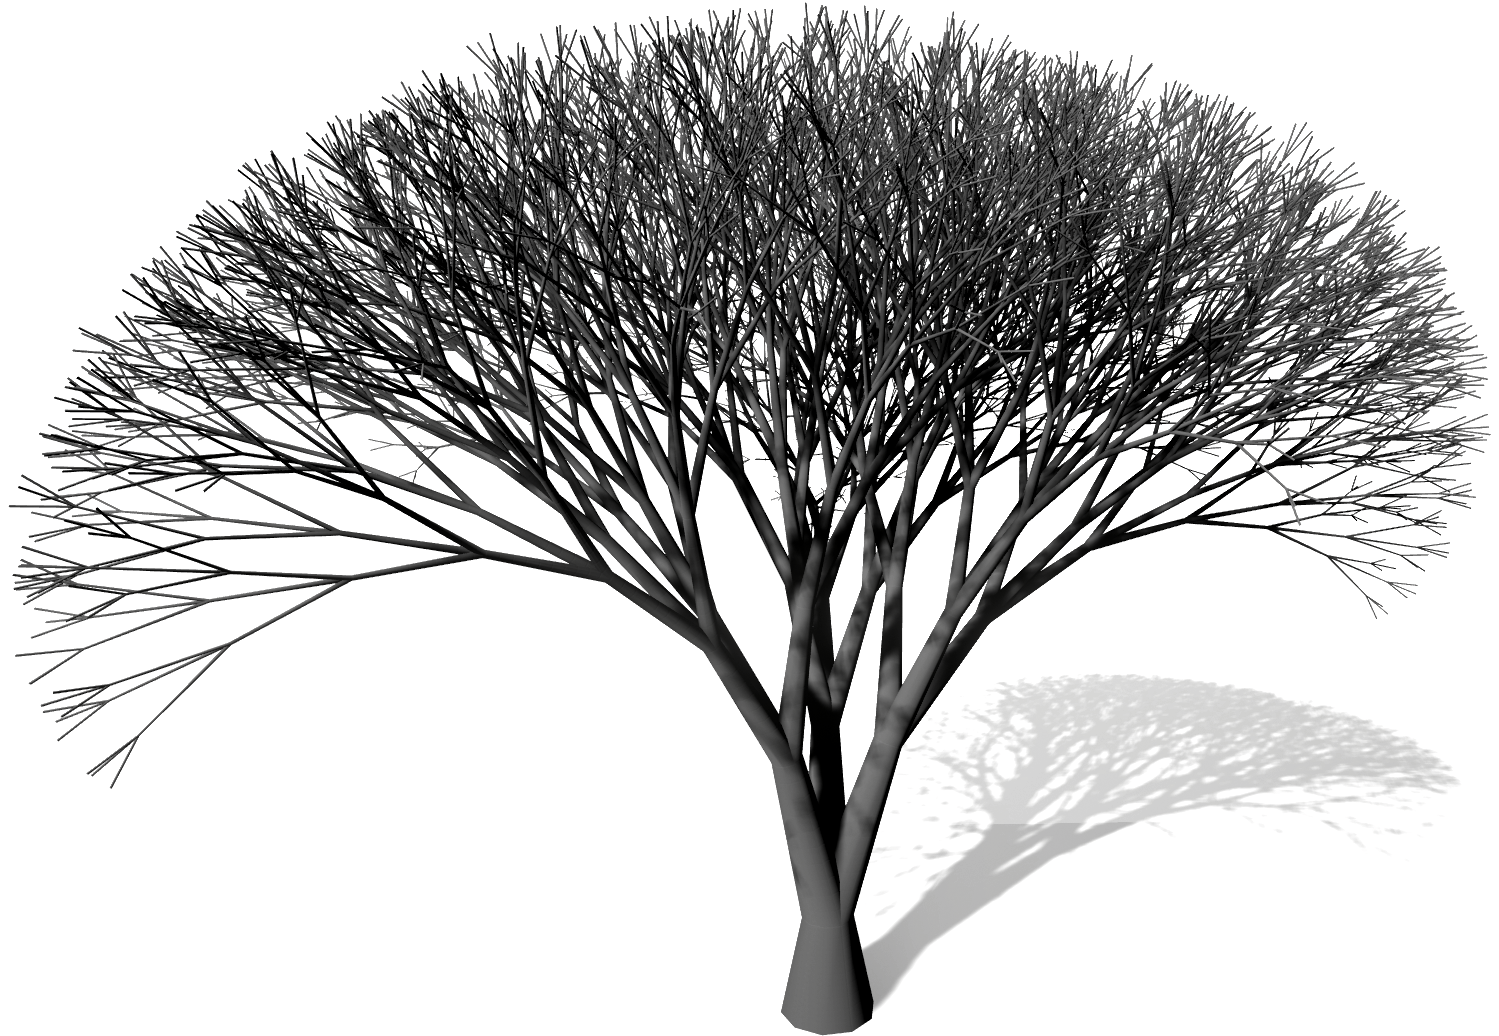
\includegraphics[width=\linewidth]{images/LS_Ternary_2.png}
		\caption{$\overrightarrow{T} = \overrightarrow{0}$, $e = 0$ \\ Entspricht Abbildung \ref{subfig:LS_Ternary_2}.}
		\label{subfig:LS_Ternary_2.2}
	\end{subfigure}
	\begin{subfigure}[t]{.45\textwidth}
		\centering
		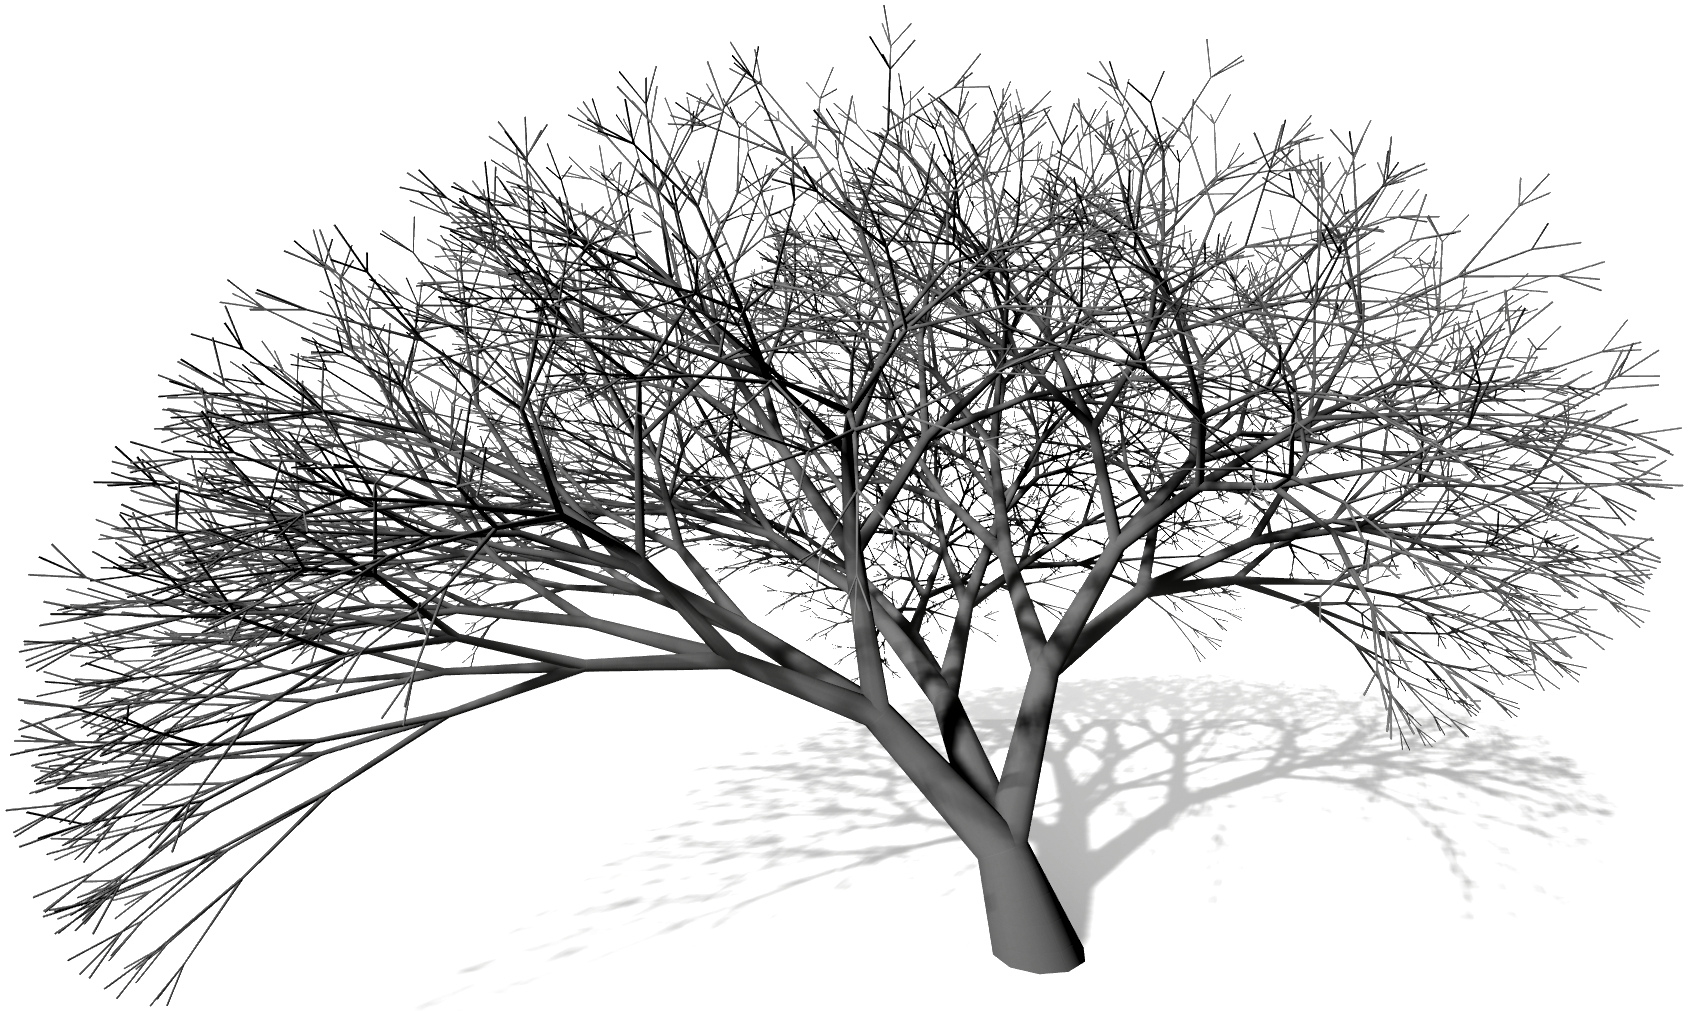
\includegraphics[width=\linewidth]{images/LS_Ternary_2_Tropism.png}
		\caption{$\overrightarrow{T} = \protect\begin{pmatrix}
			0 \\
			-0.5 \\
			-1
			\protect\end{pmatrix}$, $e = 0.5$}
		\label{subfig:LS_Ternary_2_Tropism}
	\end{subfigure}	
	\begin{subfigure}[t]{.45\textwidth}
		\centering
		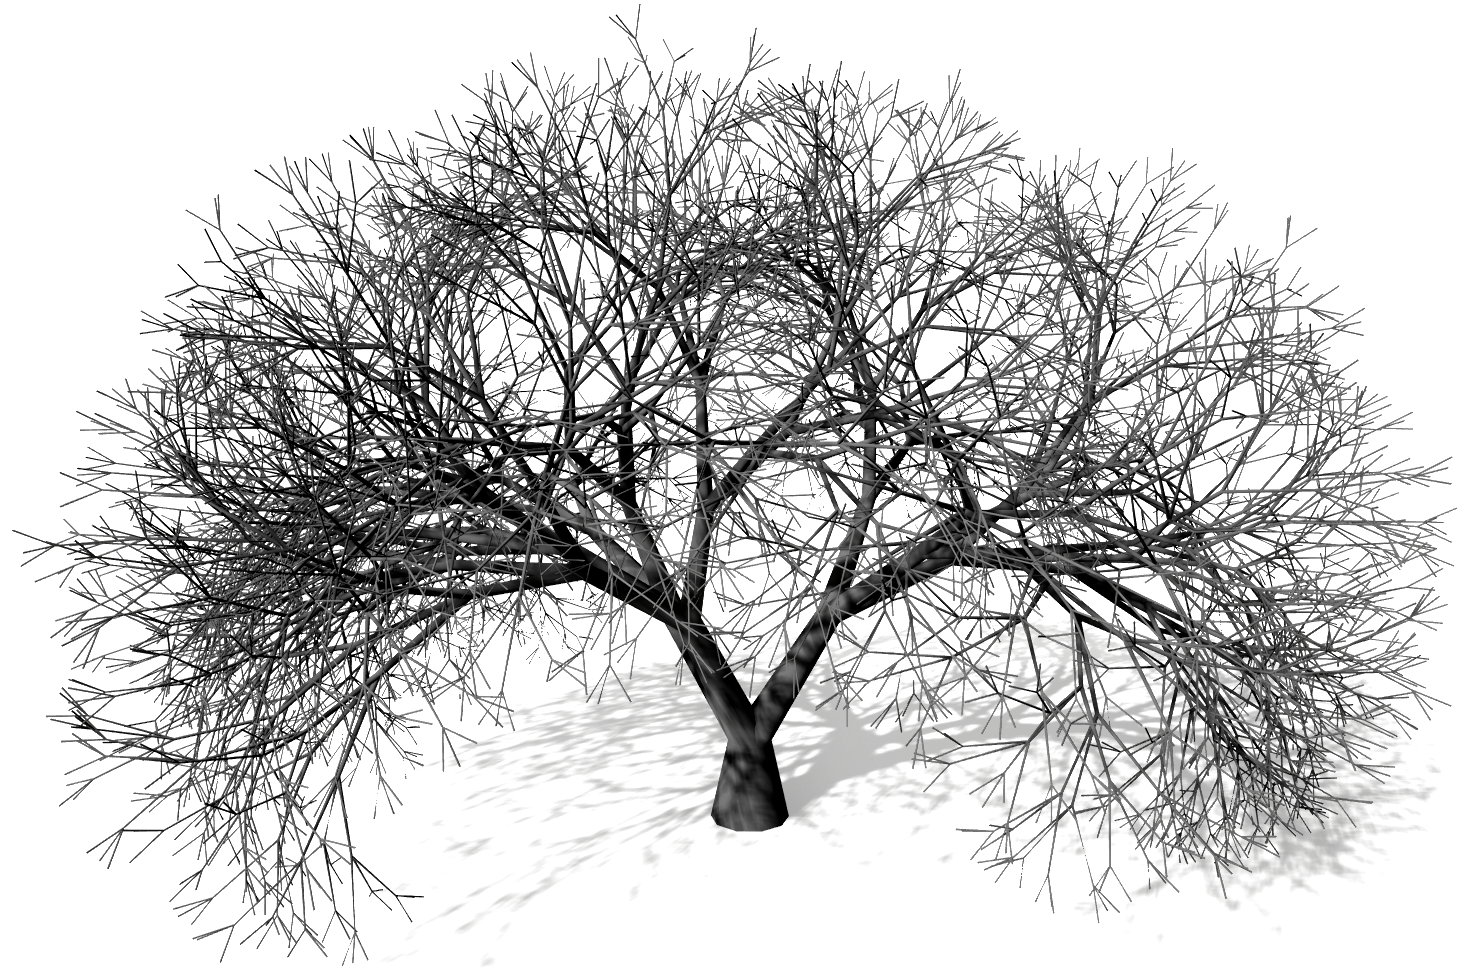
\includegraphics[width=\linewidth]{images/LS_Ternary_4.png}
		\caption{$\overrightarrow{T} = \overrightarrow{0}$, $e = 0$\\ Entspricht Abbildung \ref{subfig:LS_Ternary_4}.}
		\label{subfig:LS_Ternary_4.2}
	\end{subfigure}
	\begin{subfigure}[t]{.45\textwidth}
		\centering
		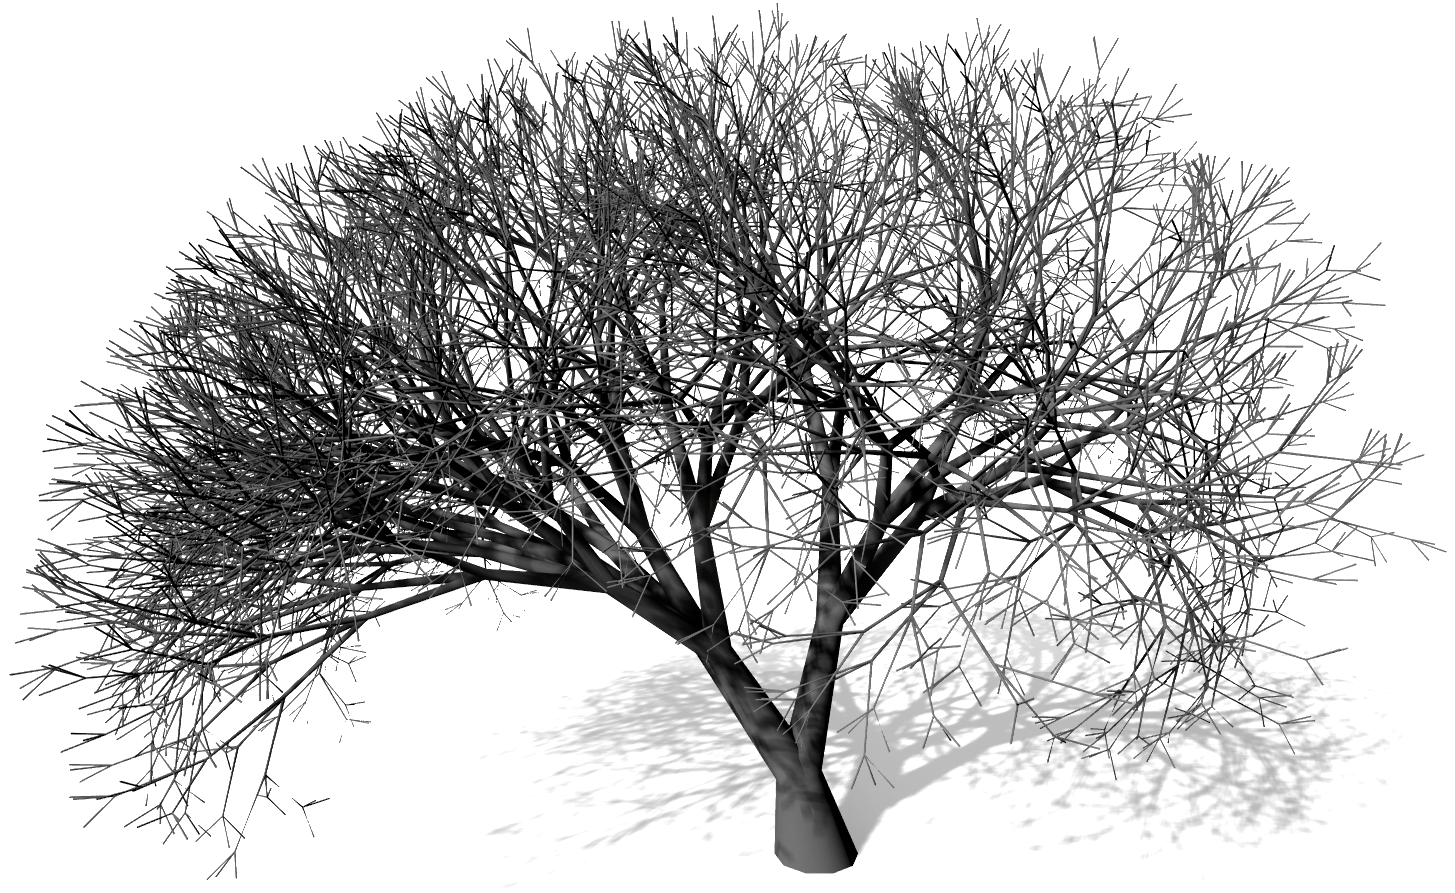
\includegraphics[width=\linewidth]{images/LS_Ternary_4_Tropism.png}
		\caption{$\overrightarrow{T} = \protect\begin{pmatrix}
			1 \\
			0 \\
			1
			\protect\end{pmatrix}$, $e = 0.3$}
		\label{subfig:LS_Ternary_4_Tropism}
	\end{subfigure}
	\caption{Beispiele ternären Wachstums mit und ohne Einfluss durch Tropismus. Entspricht der n-fachen Ableitung des Axioms anhand der Produktionsregeln aus Gleichung \ref{eq:ProdTernary}. Die linken und rechten Abbildungen unterscheiden sich jeweils im Tropismusvektor $\protect\overrightarrow{T}$ und im Biegsamkeitsfaktor $e$. Eigene Abbildungen.}
	\label{fig:LS_Ternary_Tropism}
\end{figure}

\section{Space-Colonization-Actor}

Die Space-Colonization Implementierung ermöglicht es durch die Angabe einiger weniger Parameter eine Vielzahl verschiedener Baumstrukturen zu generieren. \cite[S.3]{SpaceColonizationAlgorithm:07} Im Folgenden wird der Einfluss dieser Parameter auf die Ergebnisse untersucht. Es werden jeweils sich unterscheidende Parameterwerte angegeben.

\subsection{Einflussbereiche}

Die Verteilung und Anzahl der Einflusspunkte hat starke Auswirkungen auf die sich ergebende Baumstruktur. Je weniger Einflusspunkte existieren, desto größer ist die Wirkung jedes Punktes auf die Position der neuen Knotenpunkte und resultiert in einer spärlich bewachsenen Baumkrone mit kantigen, ungleichmäßig verteilten Ästen. Wird die Anzahl der Einflusspunkte erhöht, entsteht eine dicht bewachsene Baumkrone mit leicht kurvenförmigen, gleichmäßig verteilten Ästen. \cite[S.3]{SpaceColonizationAlgorithm:07}

Weiterhin passt sich die generierte Baumstruktur dem Bereich an, in welchem die Einflusspunkte generiert werden. Es können entweder einzelne Bereichprimitive, wie eine Kugel- oder Zylinderform, oder mehrere miteinander verknüpfte Einflussbereiche verwendet werden. \cite[S.4]{SpaceColonizationAlgorithm:07}

\begin{figure} [hbtp]
	\centering
	\begin{subfigure}[t]{.45\textwidth}
		\centering
		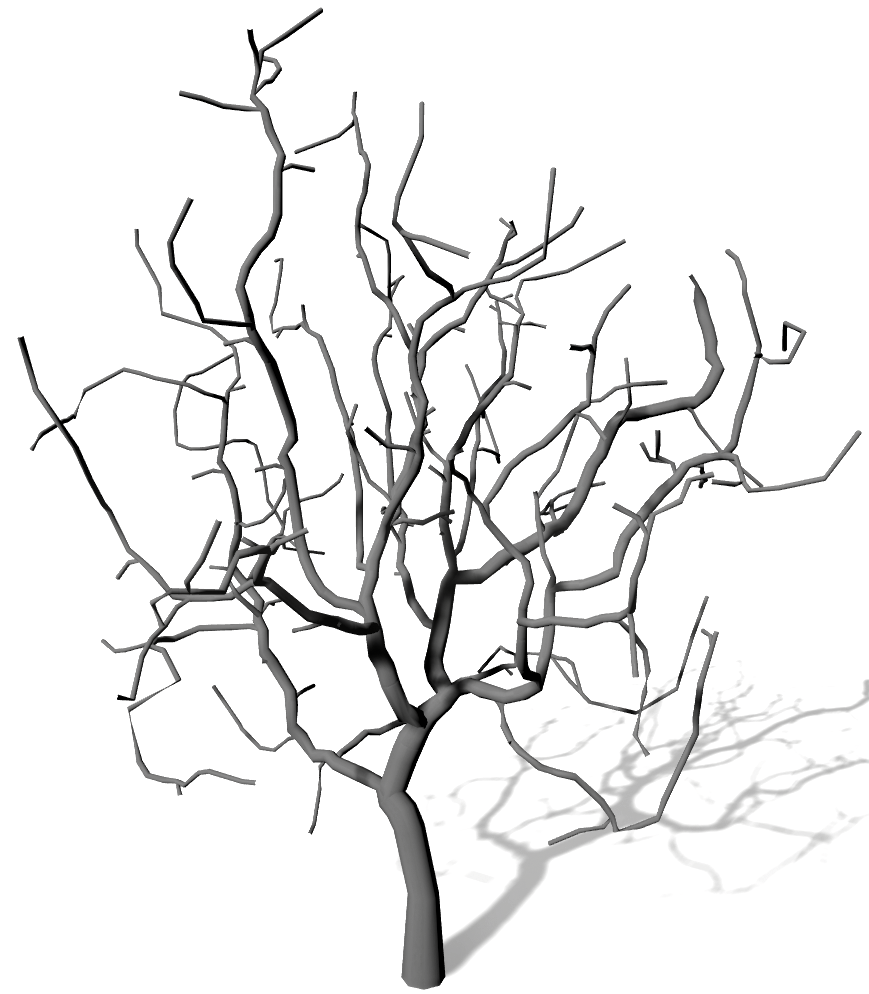
\includegraphics[height=.21\textheight]{images/SCA_Einfluss_Sphere_Low.png}
		\caption{Kugelförmig mit Radius $r = 500$, $N = 1000$}
		\label{subfig:SCA_Einfluss_Sphere_Low}
	\end{subfigure}
	\hspace{.05\linewidth}
	\begin{subfigure}[t]{.45\textwidth}
		\centering
		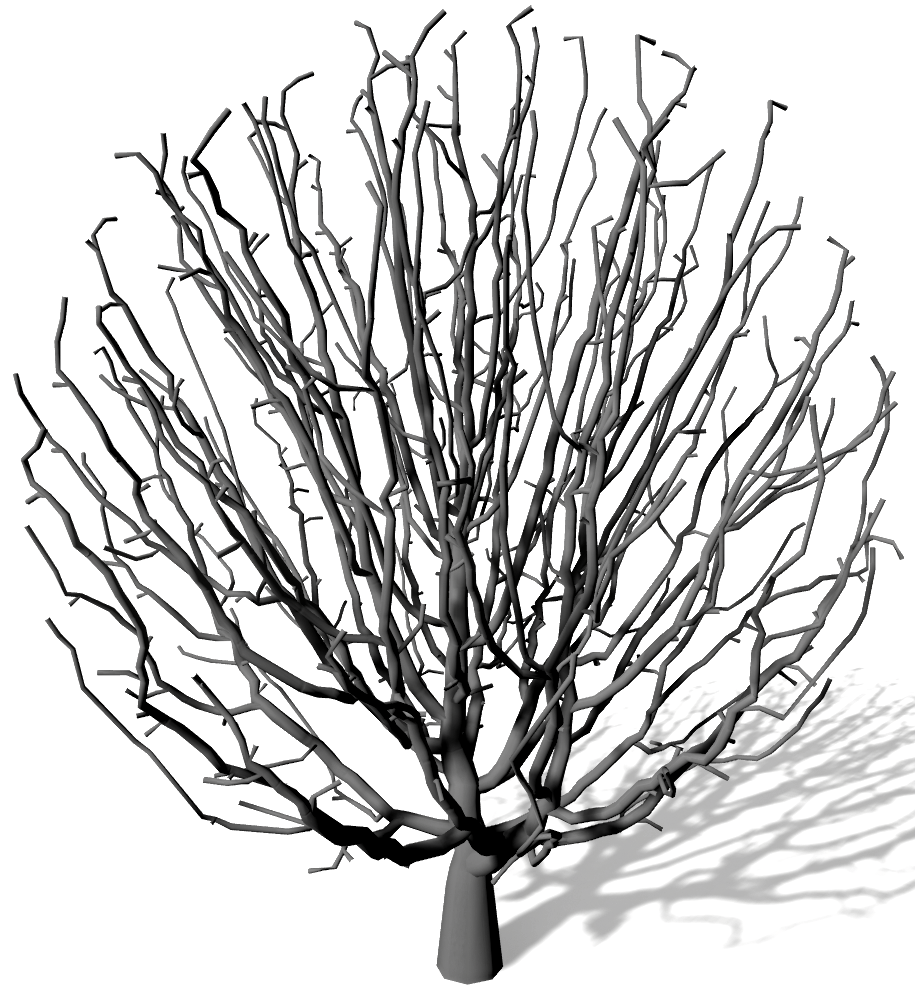
\includegraphics[height=.21\textheight]{images/SCA_Einfluss_Sphere_High.png}
		\caption{Kugelförmig mit Radius $r = 500$, $N = 10000$}
		\label{subfig:SCA_Einfluss_Sphere_High}
	\end{subfigure}	
	\begin{subfigure}[t]{.45\textwidth}
		\centering
		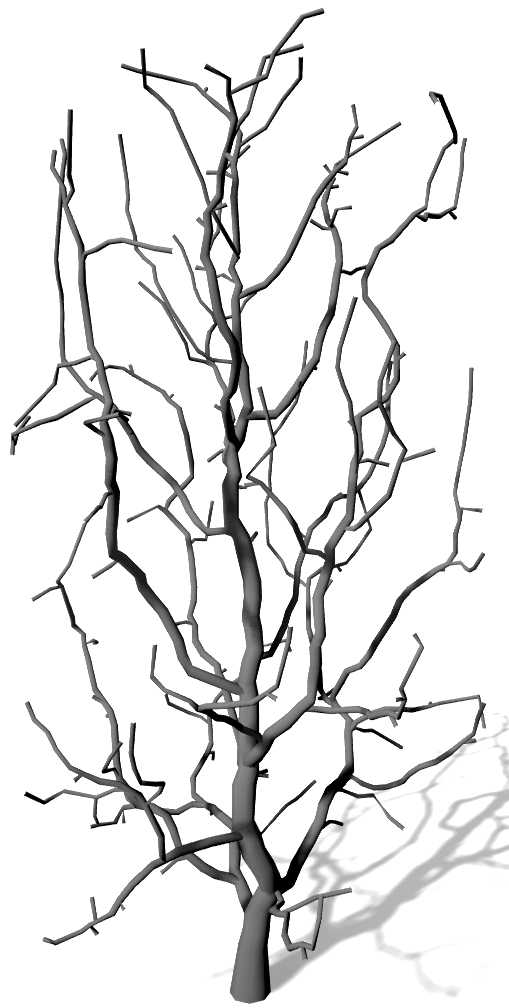
\includegraphics[height=.21\textheight]{images/SCA_Einfluss_Cylinder_Low.png}
		\caption{Zylinderförmig mit Höhe $h=1000$ und Radius $r_z = 300$, $N = 1000$}
		\label{subfig:SCA_Einfluss_Cylinder_Low}
	\end{subfigure}
	\hspace{.05\linewidth}
	\begin{subfigure}[t]{.45\textwidth}
		\centering
		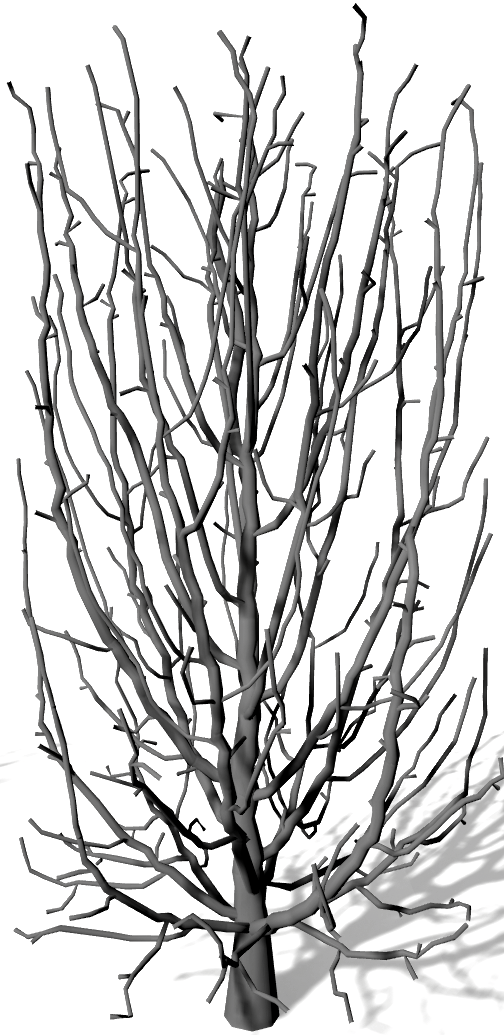
\includegraphics[height=.21\textheight]{images/SCA_Einfluss_Cylinder_High.png}
		\caption{Zylinderförmig mit Höhe $h=1000$ und Radius $r_z = 300$, $N = 10000$}
		\label{subfig:SCA_Einfluss_Cylinder_High}
	\end{subfigure}
	\caption{Wirkung der Anzahl der Einflusspunkte $N$ und der Form des Einflussbereichs auf die generierte Baumstruktur. Eigene Abbildungen.}
	\label{fig:SCA_Einfluss}
\end{figure}
 
 \begin{figure} [hbtp]
 	\centering
 	\begin{subfigure}[t]{.45\textwidth}
 		\centering
 		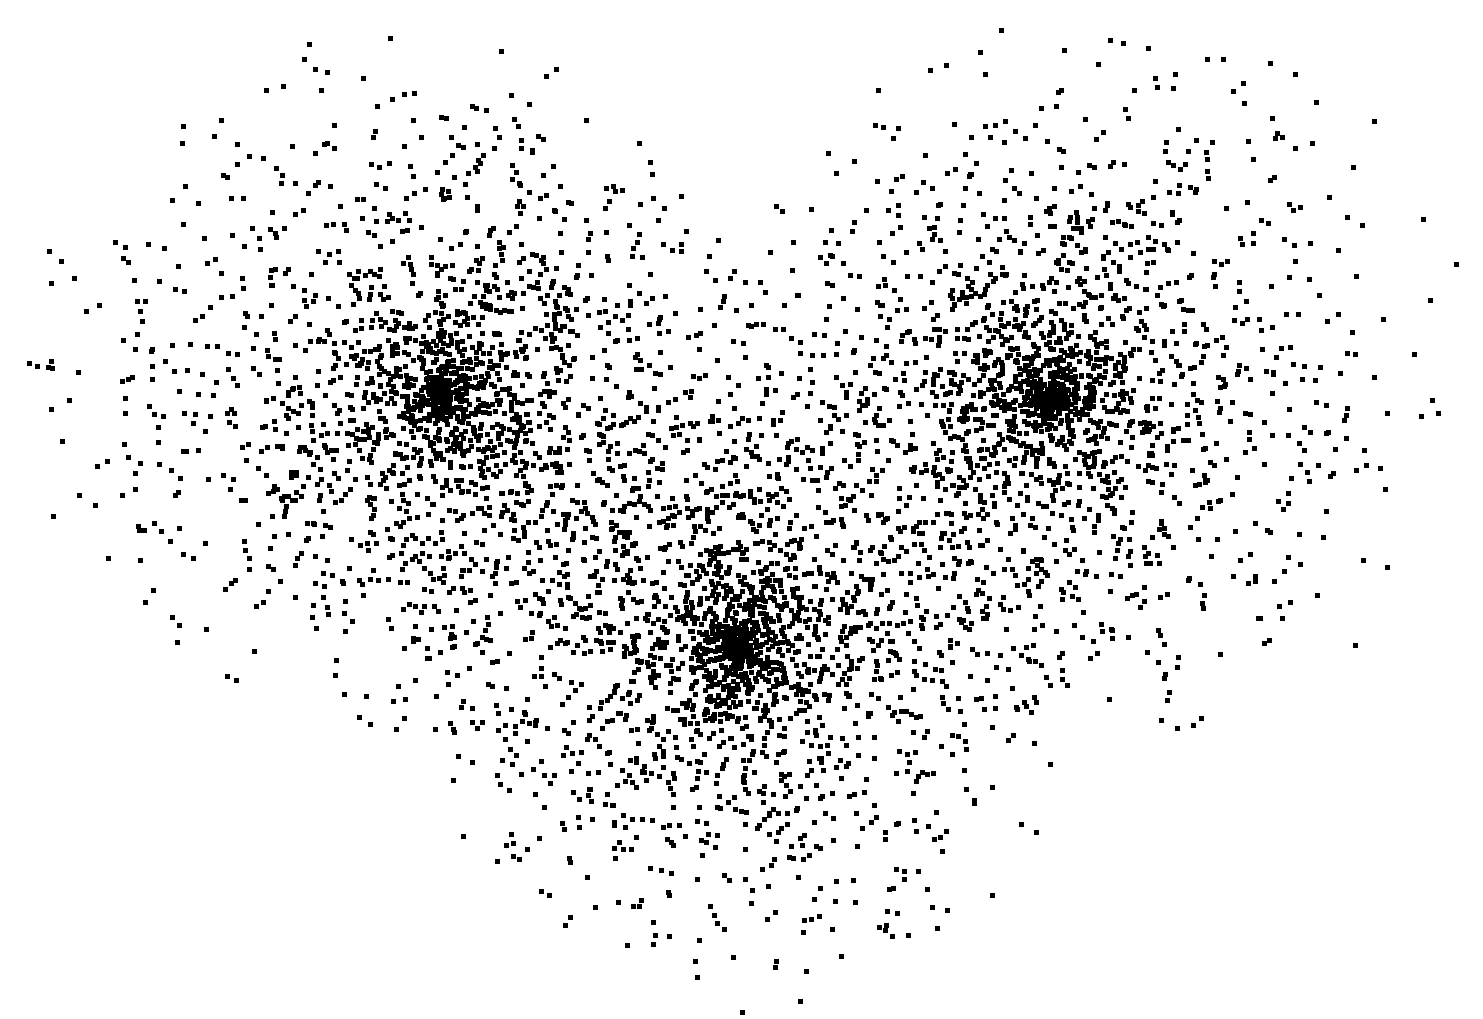
\includegraphics[height=.19\textheight]{images/SCA_MultipleSpheres_Points.png}
 		\caption{Punktewolke.}
 		\label{subfig:SCA_MultipleSpheres_Points}
 	\end{subfigure}
 	\hspace{.05\linewidth}
 	\begin{subfigure}[t]{.45\textwidth}
 		\centering
 		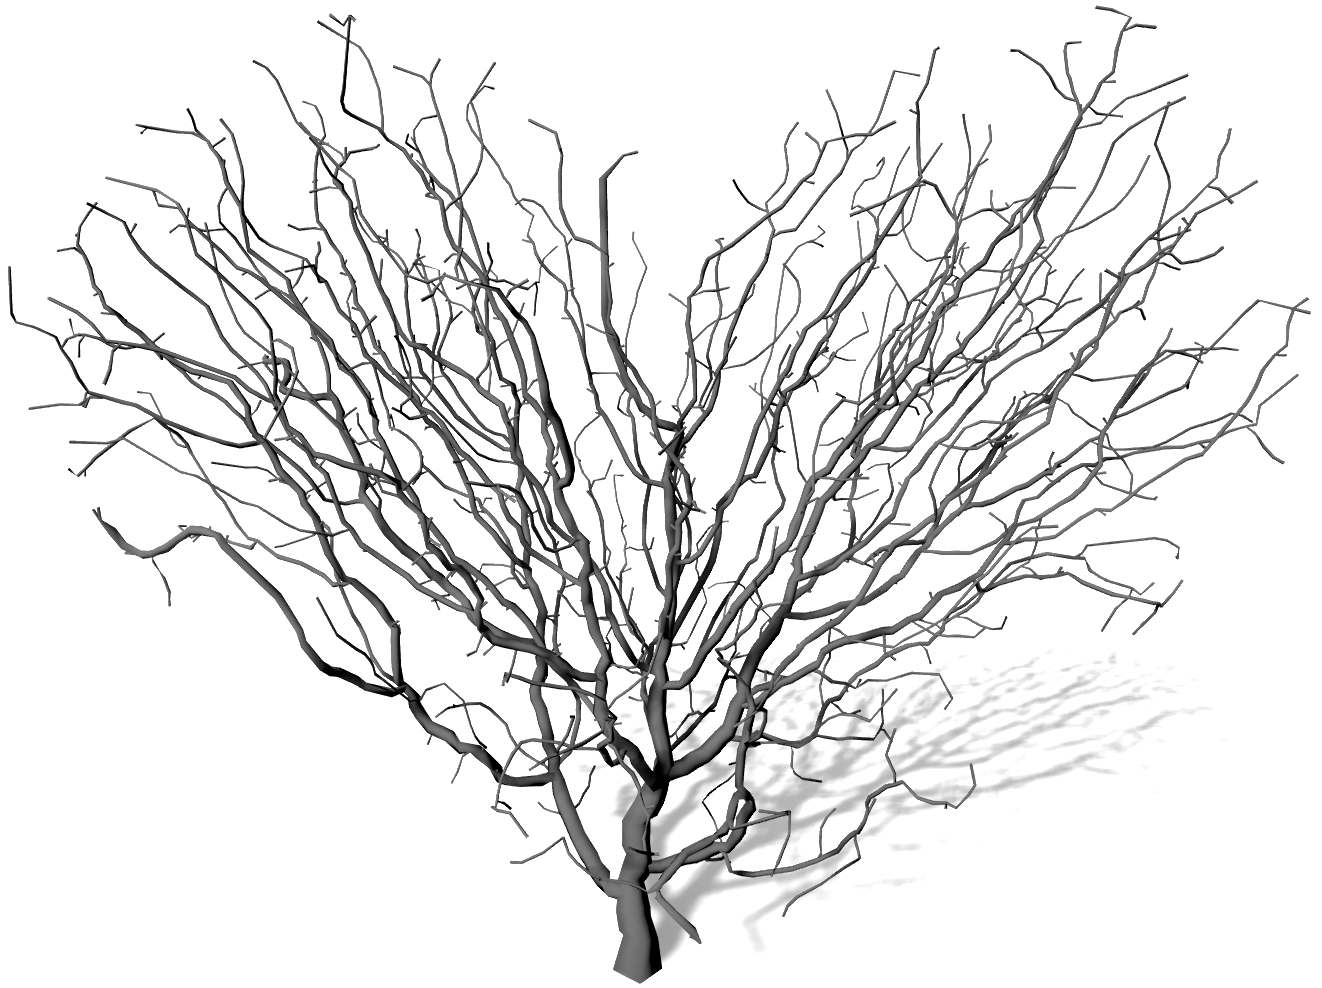
\includegraphics[height=.19\textheight]{images/SCA_MultipleSpheres_Grown.png}
 		\caption{Resultierende Baumstruktur.}
 		\label{subfig:SCA_MultipleSpheres_Grown}
 	\end{subfigure}	
 	\caption{Verbindung von drei kugelförmigen Einflussbereichen zu einem Bereich. Die Kugeln haben jeweils den Radius $r=500$ und $N=2000$. Eigene Abbildungen.}
 	\label{fig:SCA_MultipleSpheres}
 \end{figure}
 
\subsection{Wachstumsparameter}

Bei den Parametern, welche sich direkt auf die Positionierung neuer Knoten auswirken, handelt es sich um Minimalradius, Einflussradius, Schrittweite, Tropismus, Maximale Zweigtiefe, gewichtetes Wachstum, den maximalen Grad eines Knotens und die maximale Anzahl von durchgeführten Iterationen.

\paragraph{Minimalradius und Einflussradius}

Der Minimalradius $d_k$ hat eine ähnliche Wirkung auf eine generierte Baumstruktur wie die Anzahl der Einflusspunkte $N$. Je höher der Minimalradius $d_k$, desto weniger Abzweigungen werden gebildet, da nach der Bildung eines neuen Astsegments Einflusspunkte entfernt werden, die zuvor eine solche Abzweigung bewirkt hätten. Die Baumkrone erscheint spärlicher bewachsen, die entstandenen Äste sind jedoch kurvenreicher, da auf die wenigen wachsenden Äste mehr Einflusspunkte einwirken -- das Entfernen oder Hinzufügen einzelner Einflusspunkte hat somit nur eine kleine Auswirkung auf die Position eines in der nächsten Iteration neu hinzugefügten Astsegments. \cite[S.3]{SpaceColonizationAlgorithm:07}

Je kleiner der Einflussradius $d_i$, desto knorriger wirkt ein Baum, da Astsegmente in jedem Iterationsschritt in den Wirkungsbereich eines Einflusspunktes geraten und diesen im nächsten Schritt wieder verlassen. \cite[S.4]{SpaceColonizationAlgorithm:07}

Abbildung \ref{fig:SCA_KDRI} zeigt Beispiele der Auswirkung unterschiedlicher Werte für Einflussradius und Minimalradius.

\begin{figure} [hbtp]
	\centering
	\begin{subfigure}[t]{.45\textwidth}
		\centering
		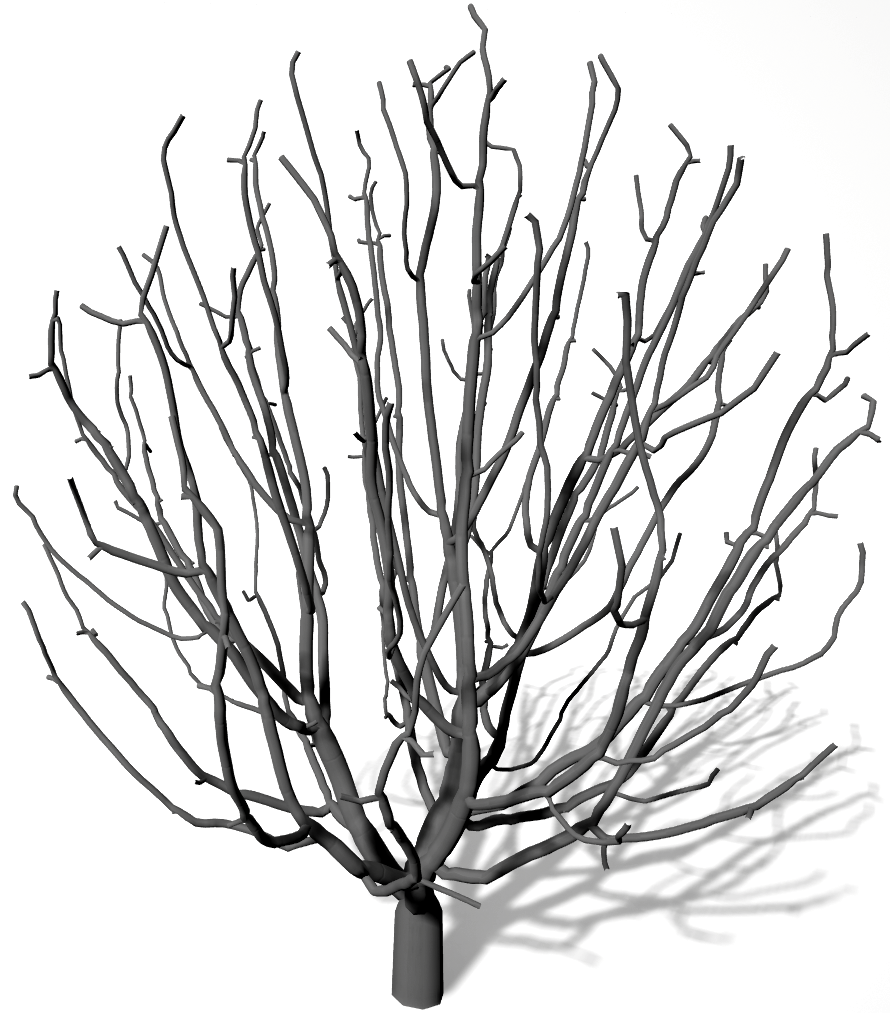
\includegraphics[height=.21\textheight]{images/SCA_KDRI_LowKD_LowRI.png}
		\caption{$d_k = 80$, $d_i = 150$}
		\label{subfig:SCA_KDRI_LowKD_LowRI}
	\end{subfigure}
	\hspace{.05\linewidth}
	\begin{subfigure}[t]{.45\textwidth}
		\centering
		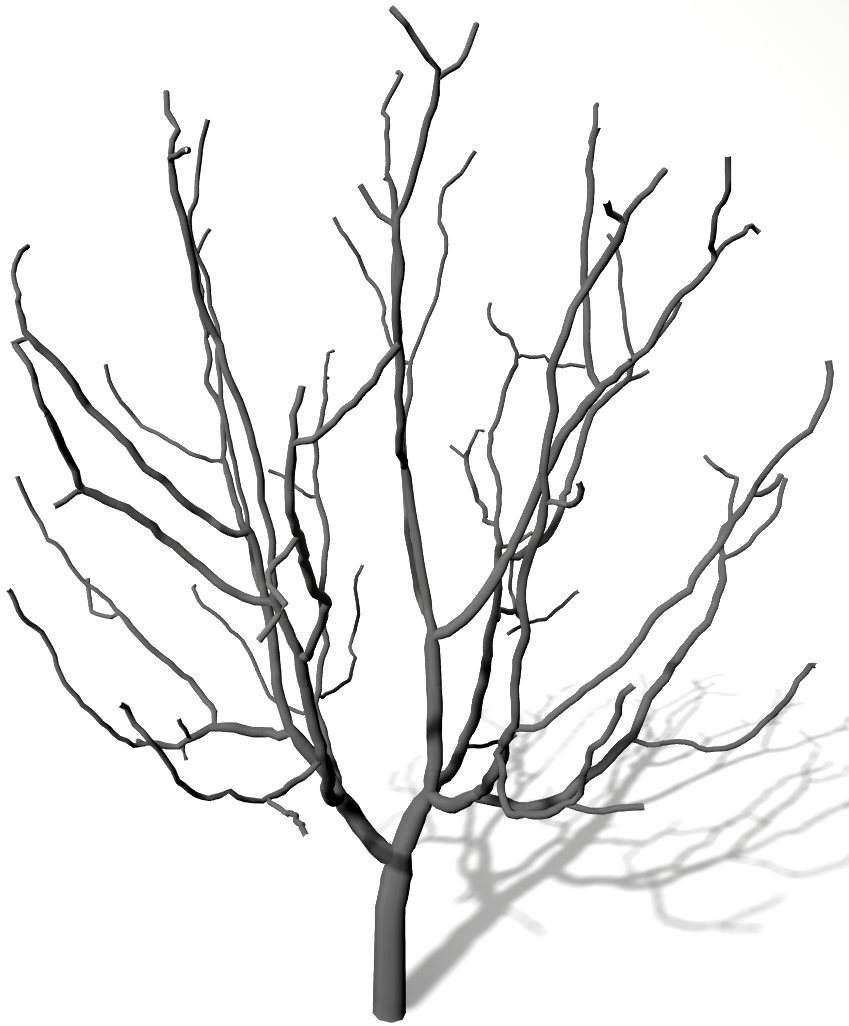
\includegraphics[height=.21\textheight]{images/SCA_KDRI_HighKD_LowRI.png}
		\caption{$d_k = 130$, $d_i = 150$}
		\label{subfig:SCA_KDRI_HighKD_LowRI}
	\end{subfigure}	
	\begin{subfigure}[t]{.45\textwidth}
		\centering
		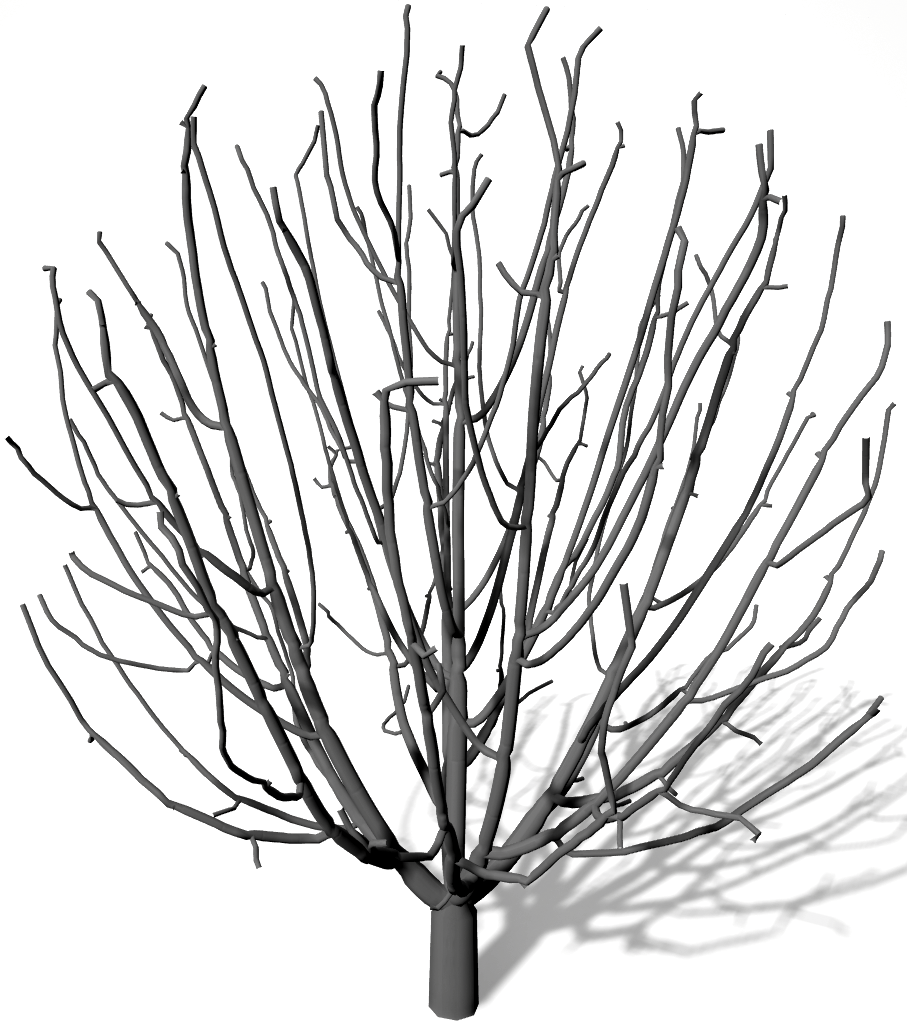
\includegraphics[height=.21\textheight]{images/SCA_KDRI_LowKD_HighRI.png}
		\caption{$d_k = 80$, $d_i = 1000$}
		\label{subfig:SCA_KDRI_LowKD_HighRI}
	\end{subfigure}
	\hspace{.05\linewidth}
	\begin{subfigure}[t]{.45\textwidth}
		\centering
		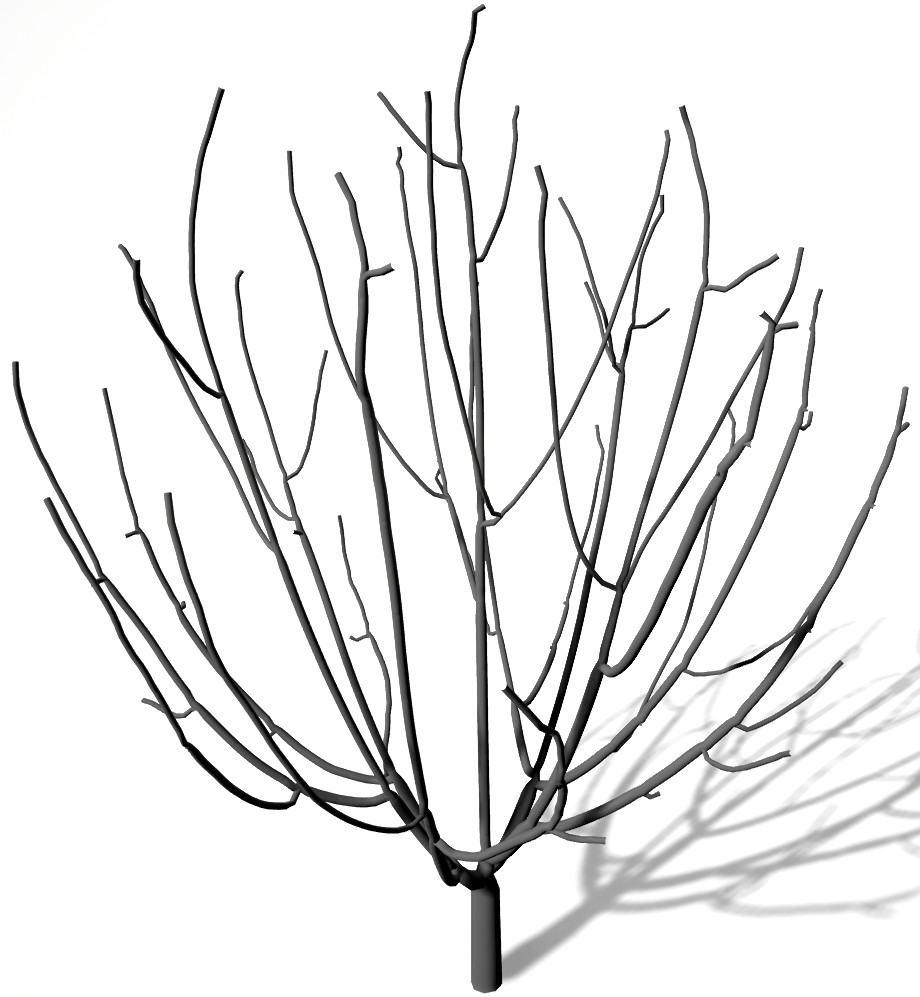
\includegraphics[height=.21\textheight]{images/SCA_KDRI_HighKD_HighRI.png}
		\caption{$d_k = 130$, $d_i = 1000$}
		\label{subfig:SCA_KDRI_HighKD_HighRI}
	\end{subfigure}
	\caption{Wirkung von Einflussradius $d_i$ und Minimalradius $d_k$ auf die generierte Baumstruktur. Es wurde die Schrittweite $D = 10$ verwendet. Eigene Abbildungen.}
	\label{fig:SCA_KDRI}
\end{figure}

\paragraph{Tropismus, maximale Zweigtiefe, maximaler Grad und gewichtetes Wachstum}

Ebenso wie bei der Implementierung von L-Systemen kann der Einfluss eines Tropismusvektors $\overrightarrow{T}$ das Wachstumsverhalten der Space-Colonization Implementierung bei gleichen Parameterwerten stark in eine bestimmte Richtung beeinflussen. Werte auf der horizontalen Ebene erwecken den Anschein von Einwirkung durch Wind. Positive Werte auf der Z-Achse entsprechen dem Streben einer Pflanze der Sonnenposition entgegen zu wachsen, negative Werte auf der Z-Achse simulieren die Einwirkung auf das Wachstum durch Gravitation. \cite[S.5]{SpaceColonizationAlgorithm:07}

Die maximale Zweigtiefe $max_Z$ begrenzt die Anzahl der Abzweigungen, die von dem Wurzel-Astsegment ausgehend zu jedem Astsegment ohne Nachfolger gebildet werden können. Bei niedrigen Werten führt dies zur Bildung weniger, kurvenförmiger Astsegmente.

Der maximale Grad $max_{grad}$ begrenzt die Anzahl der Abzweigungen, die von einem einzelnen Astsegment ausgehen können. Da Astsegmente nur in sehr dichten Baumstrukturen -- Strukturen mit vielen Einflusspunkten und einem niedrigen Minimalradius -- mehr als zwei Nachfolger bilden, hat dieser Parameter eine eingeschränkte visuelle Einwirkung. In dichten Baumstrukturen ermöglicht er es jedoch, bei minimaler visueller Einwirkung, die Anzahl der erstellten Vertizes zu begrenzen. Die Wahl von $max_{grad} = 1$ sorgt für die Bildung eines durchgängigen, in sich verdrehten Astes ohne Abzweigungen.

In Abbildung \ref{fig:SCA_Sonst} werden Beispiele für die Wirkung der beschriebenen Parameter gezeigt.

\begin{figure} [hbtp]
	\centering
	\begin{subfigure}[t]{.45\textwidth}
		\centering
		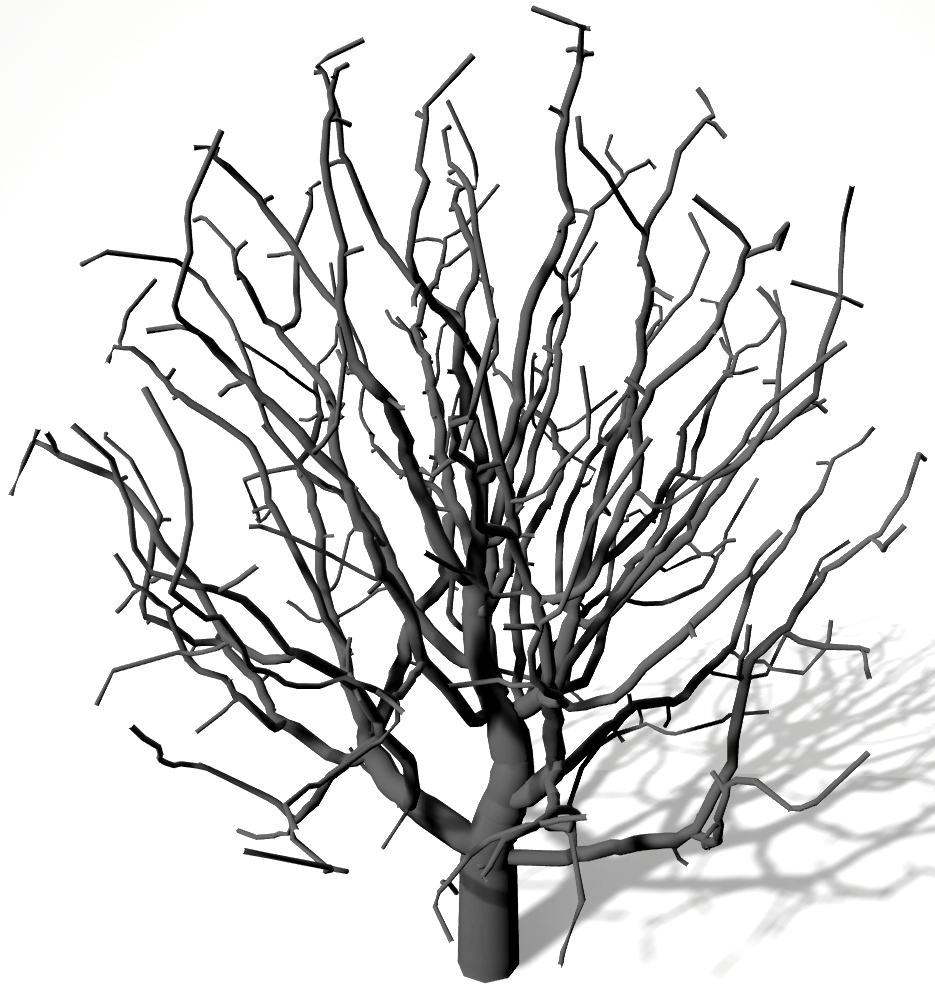
\includegraphics[height=.21\textheight]{images/SCA_Sonst_Ursprung.png}
		\caption{$d_k = 60$, $d_i = 150$, $\protect\overrightarrow{T} = (0,0,0.2)$, $r = 600$, $N = 2000$, $max_Z = 20$, $max_{grad} = 20$, kein gewichtetes Wachstum.}
		\label{subfig:SCA_Sonst_Ursprung}
	\end{subfigure}
	\hspace{.05\linewidth}
	\begin{subfigure}[t]{.45\textwidth}
		\centering
		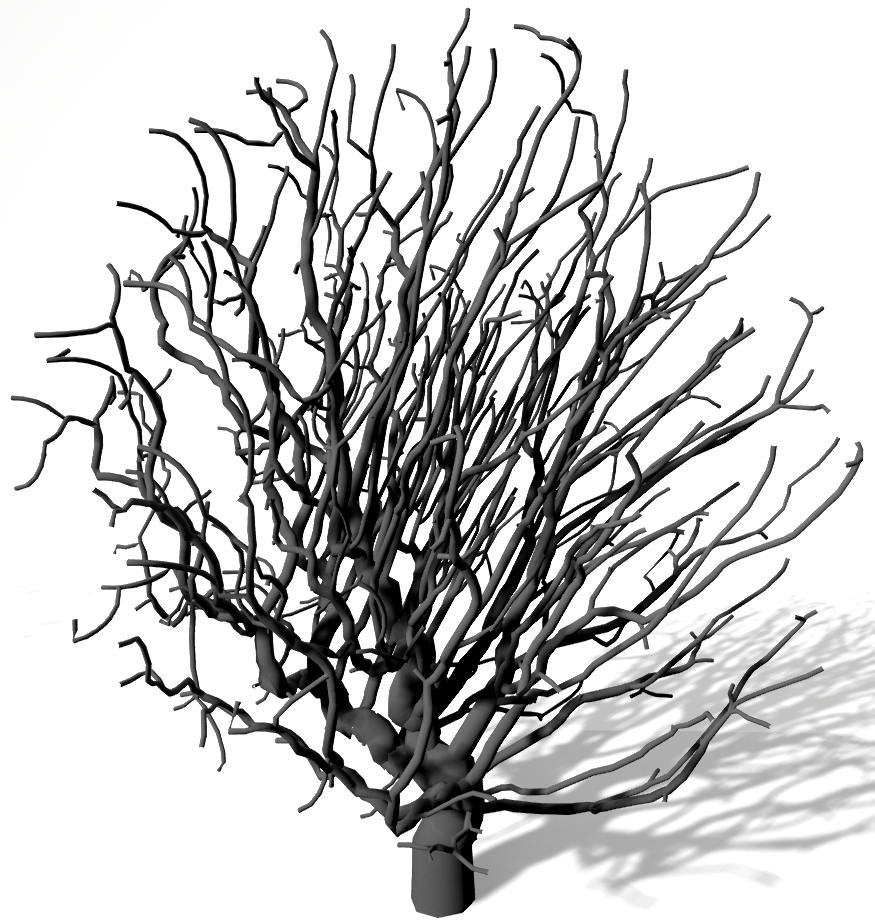
\includegraphics[height=.21\textheight]{images/SCA_Sonst_Tropism_Wind.png}
		\caption{$\protect\overrightarrow{T} = (0,0.8,0)$}
		\label{subfig:SCA_Sonst_Tropism_Wind}
	\end{subfigure}	
	\begin{subfigure}[t]{.45\textwidth}
		\centering
		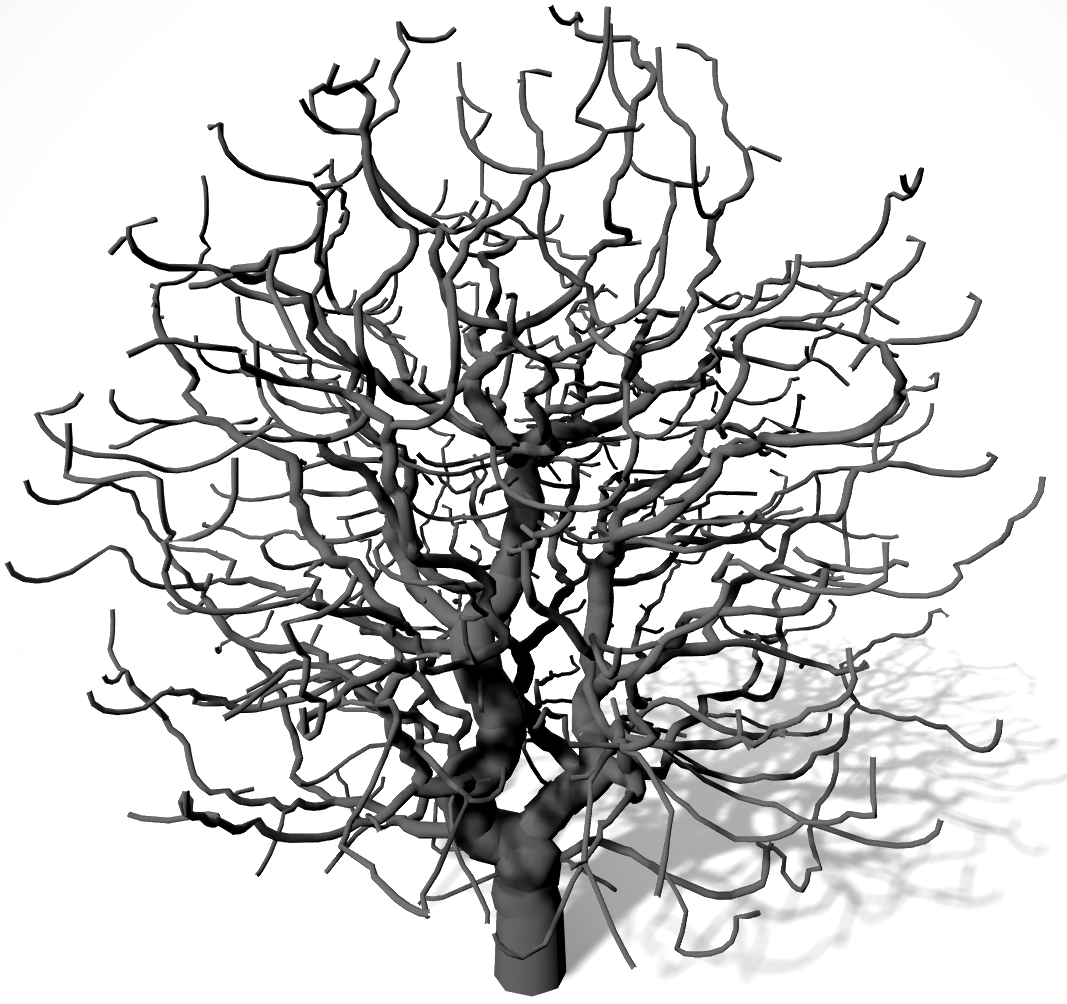
\includegraphics[height=.21\textheight]{images/SCA_Sonst_Tropism_Grav.png}
		\caption{$\protect\overrightarrow{T} = (0,0,-0.8)$}
		\label{subfig:SCA_Sonst_Tropism_Grav}
	\end{subfigure}
	\hspace{.05\linewidth}
	\begin{subfigure}[t]{.45\textwidth}
		\centering
		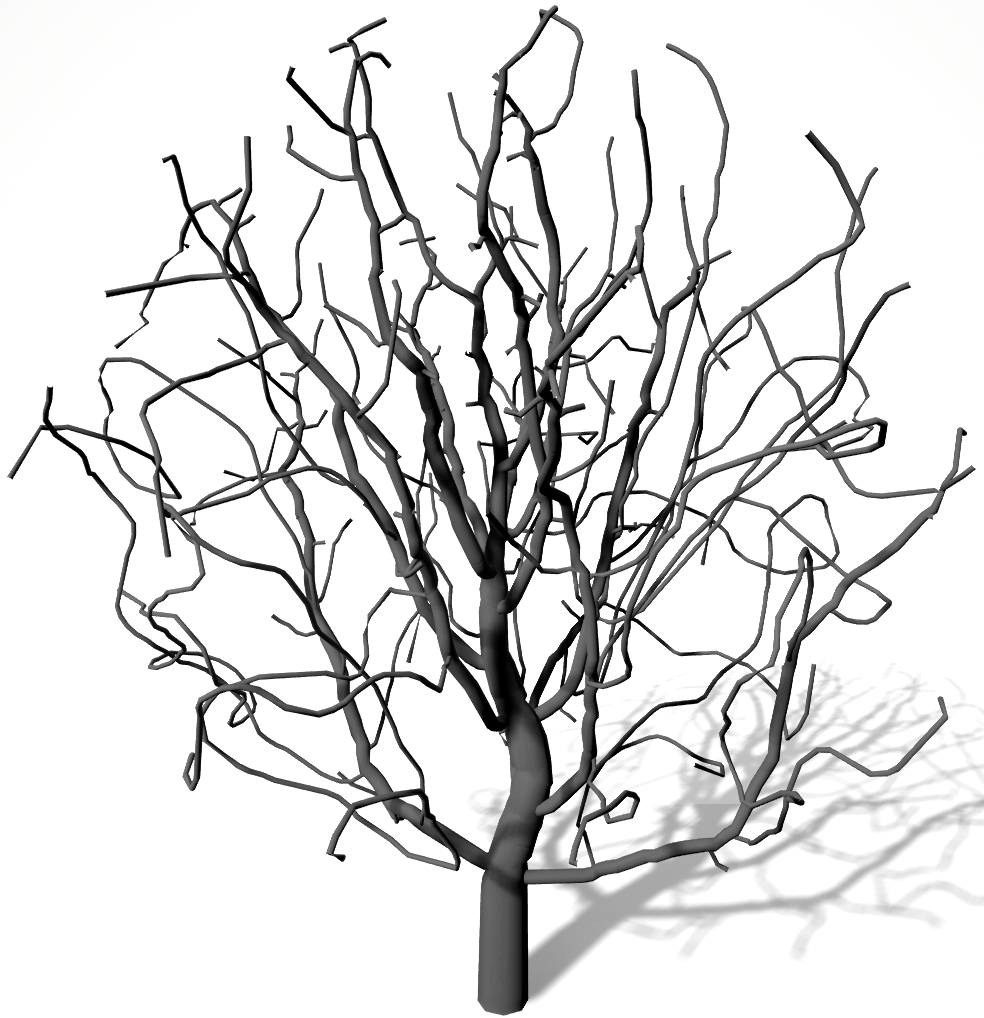
\includegraphics[height=.21\textheight]{images/SCA_Sonst_Zweigtiefe.png}
		\caption{$max_Z = 2$}
		\label{subfig:SCA_Sonst_Zweigtiefe}
	\end{subfigure}
	\begin{subfigure}[t]{.45\textwidth}
		\centering
		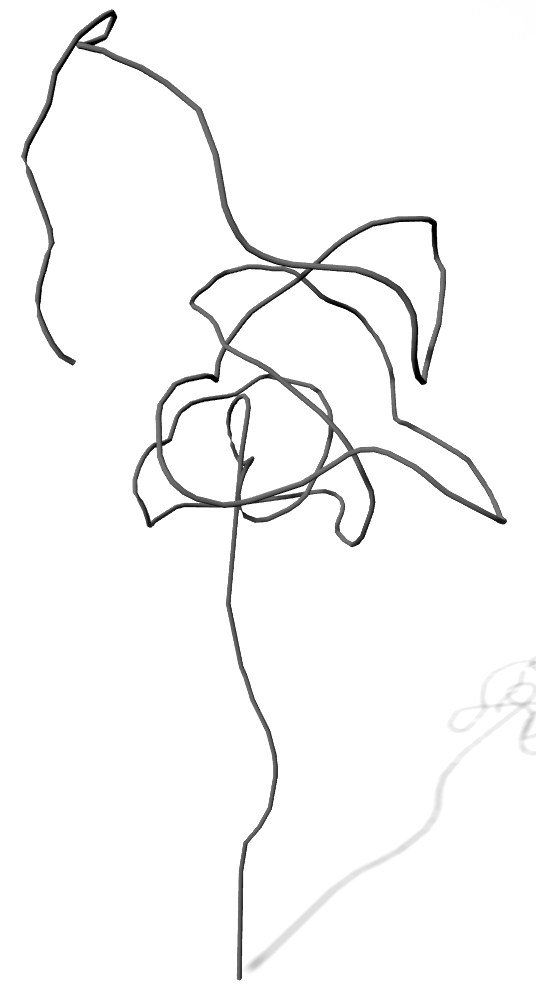
\includegraphics[height=.21\textheight]{images/SCA_Sonst_Grad.png}
		\caption{$max_{grad} = 1$}
		\label{subfig:SCA_Sonst_Grad1}
	\end{subfigure}
	\begin{subfigure}[t]{.45\textwidth}
		\centering
		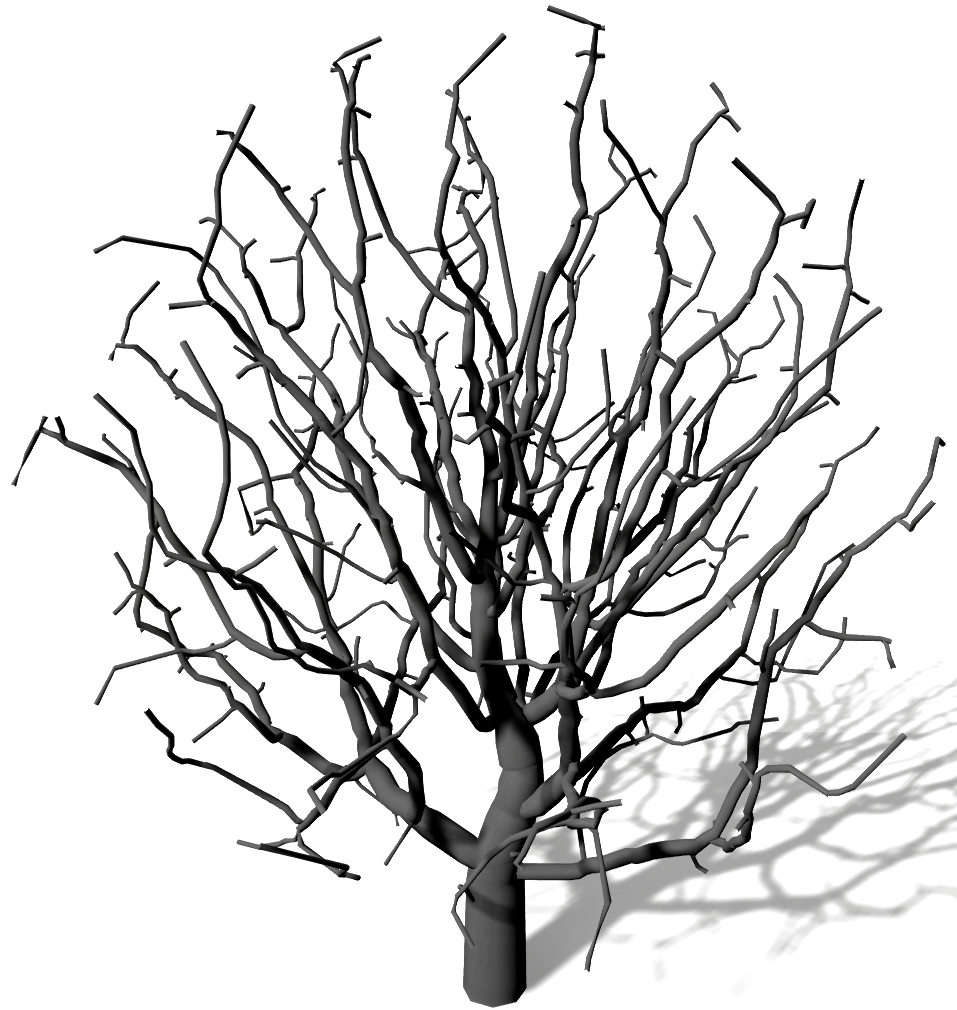
\includegraphics[height=.21\textheight]{images/SCA_Sonst_Grad2.png}
		\caption{$max_{grad} = 2$}
		\label{subfig:SCA_Sonst_Grad2}
	\end{subfigure}
	\caption{Wirkung von Tropismus $\protect\overrightarrow{T}$, maximaler Zweigtiefe $max_Z$ und maximalem Knotengrad $max_{grad}$ auf die generierte Baumstruktur. Falls nicht weiter angegeben, wurden die in Abbildung \ref{subfig:SCA_Sonst_Ursprung} angegebenen Parameterwerte verwendet. Eigene Abbildungen.}
	\label{fig:SCA_Sonst}
\end{figure}
 
\paragraph{Schrittweite und maximale Anzahl durchzuführender Iterationen}

Je höher die Schrittweite $D$, desto knorriger wirkt ein Baum -- ähnlich dem Einflussradius -- da ein Astsegment in jedem Schritt Einflussradien betritt und verlässt oder ein neues Astsegment auf der gegenüberliegenden Seite eines Einflusspunktes gebildet wird und von diesem nun aus der entgegengesetzten Richtung beeinflusst wird. Weiterhin besitzen die Äste scharfe Kanten, da aufgrund der größeren Schrittweite weniger Vertizes generiert werden. Die Wahl einer niedrigen Schrittweite führt zur Bildung von Ästen mit leichten Kurven.

Die maximale Anzahl durchzuführender Iterationen $N_I$ beschränkt die Zahl von Space-Colonization Iterationen, die durchgeführt werden sollen. Die bisher gezeigten Beispiele wurden mit $N_I = 400$ durchgeführt und vor Erreichen dieser Zahl abgebrochen. Bei Festlegung niedrigerer Zahlen kann das Wachstum des Baumes beschränkt oder das Wachstumsverhalten im Laufe der Iterationen beobachtet werden.

Abbildung \ref{fig:SCA_SI} zeigt die Auswirkungen verschiedener Werte für die Schrittweite und die maximale Anzahl durchzuführender Iterationen bei gleichbleibender Verteilung der Einflusspunkte.

\begin{figure} [hbtp]
	\centering
	\begin{subfigure}[t]{.45\textwidth}
		\centering
		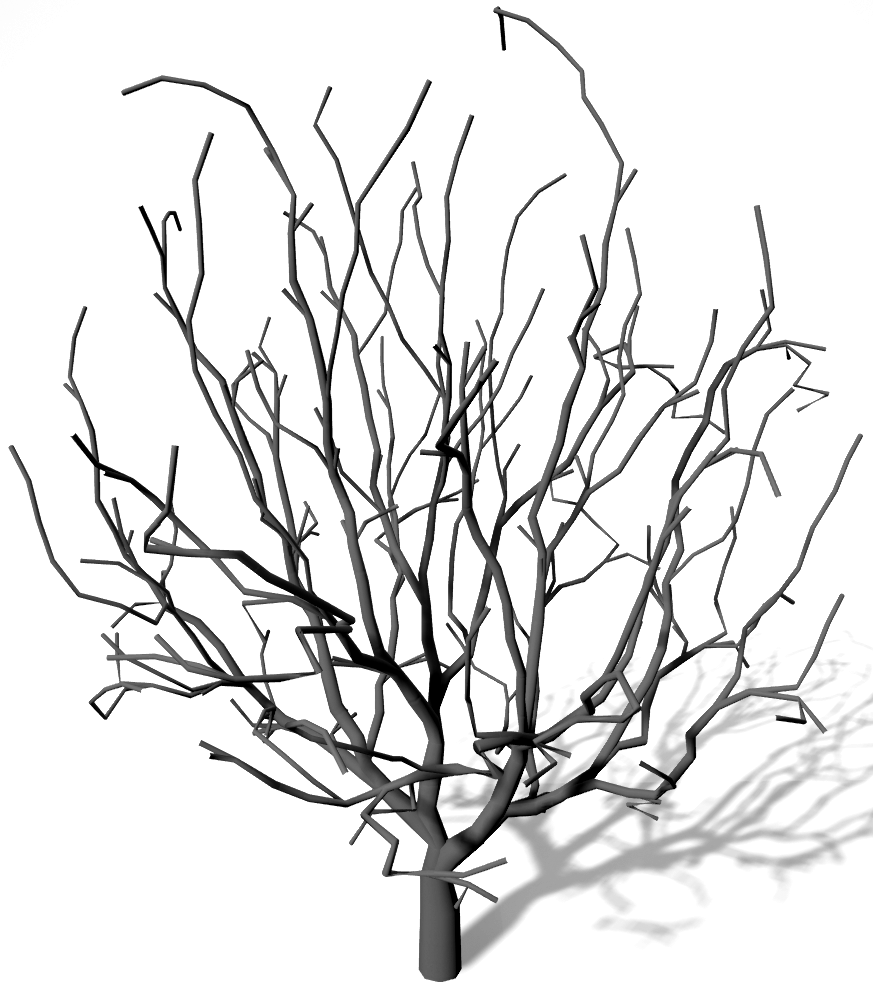
\includegraphics[height=.21\textheight]{images/SCA_SI_SchrittweiteHigh.png}
		\caption{$d_k = 100$, $d_i = 150$, $D = 50$, $N_I = 400$}
		\label{subfig:SCA_SI_SchrittweiteHigh}
	\end{subfigure}
	\hspace{.01\linewidth}
	\begin{subfigure}[t]{.45\textwidth}
		\centering
		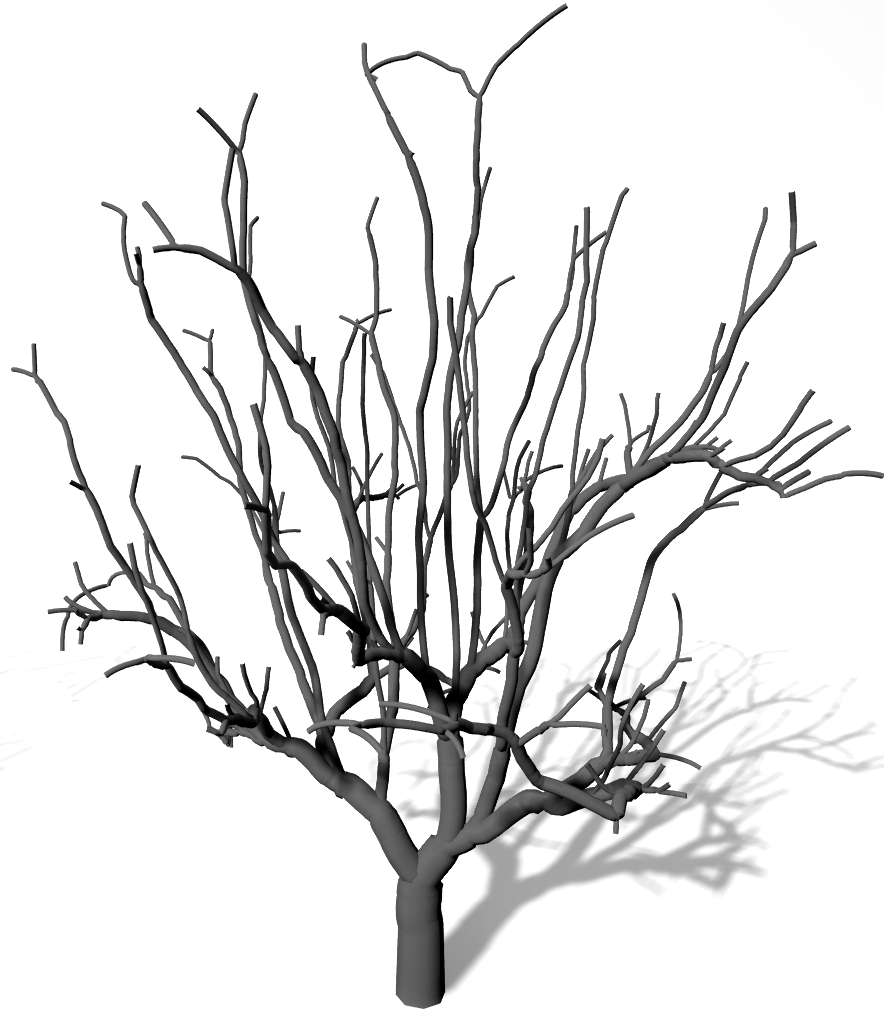
\includegraphics[height=.21\textheight]{images/SCA_SI_SchrittweiteLow.png}
		\caption{$D = 5$}
		\label{subfig:SCA_SI_SchrittweiteLow}
	\end{subfigure}	
	\begin{subfigure}[t]{.19\textwidth}
		\centering
		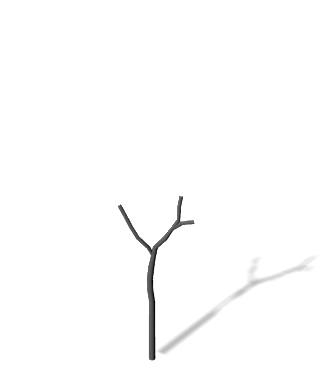
\includegraphics[height=.11\textheight]{images/SCA_SI_Iterationen10.png}
		\caption{$D = 20$, $N_I = 10$}
		\label{subfig:SCA_SI_Iterationen10}
	\end{subfigure}
	\begin{subfigure}[t]{.19\textwidth}
		\centering
		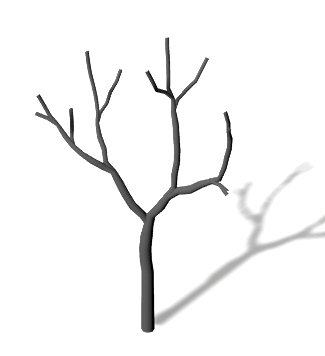
\includegraphics[height=.11\textheight]{images/SCA_SI_Iterationen20.png}
		\caption{$N_I = 20$}
		\label{subfig:SCA_SI_Iterationen20}
	\end{subfigure}
	\begin{subfigure}[t]{.19\textwidth}
		\centering
		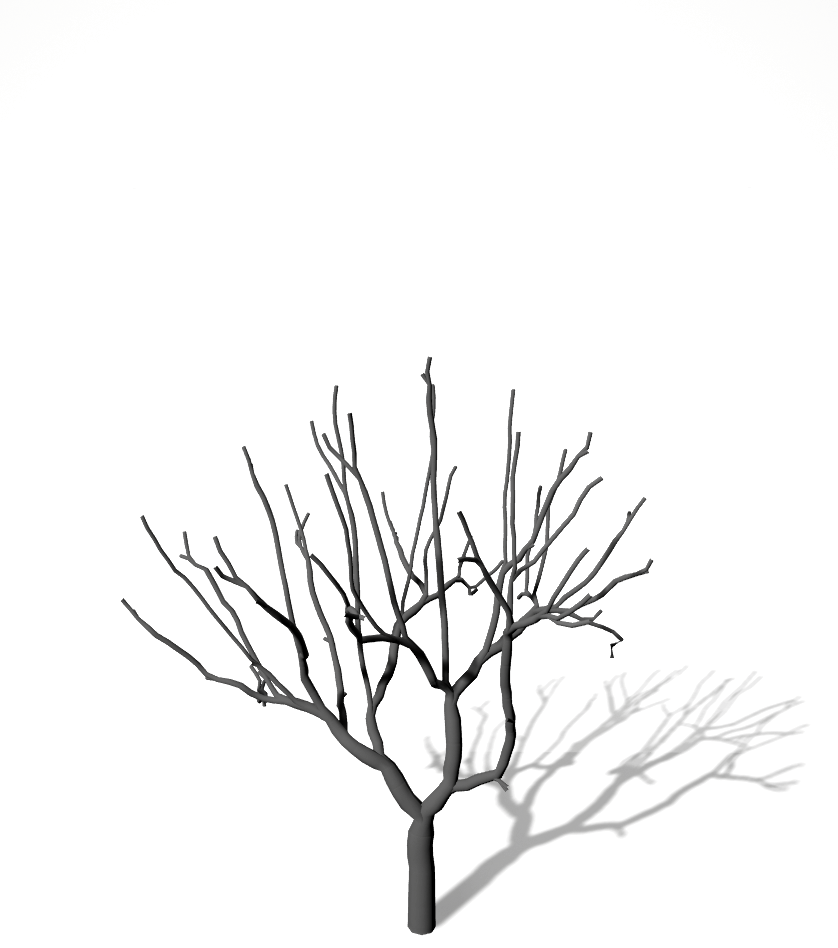
\includegraphics[height=.21\textheight]{images/SCA_SI_Iterationen40.png}
		\caption{$N_I = 40$}
		\label{subfig:SCA_SI_Iterationen40}
	\end{subfigure}
	\begin{subfigure}[t]{.4\textwidth}
		\centering
		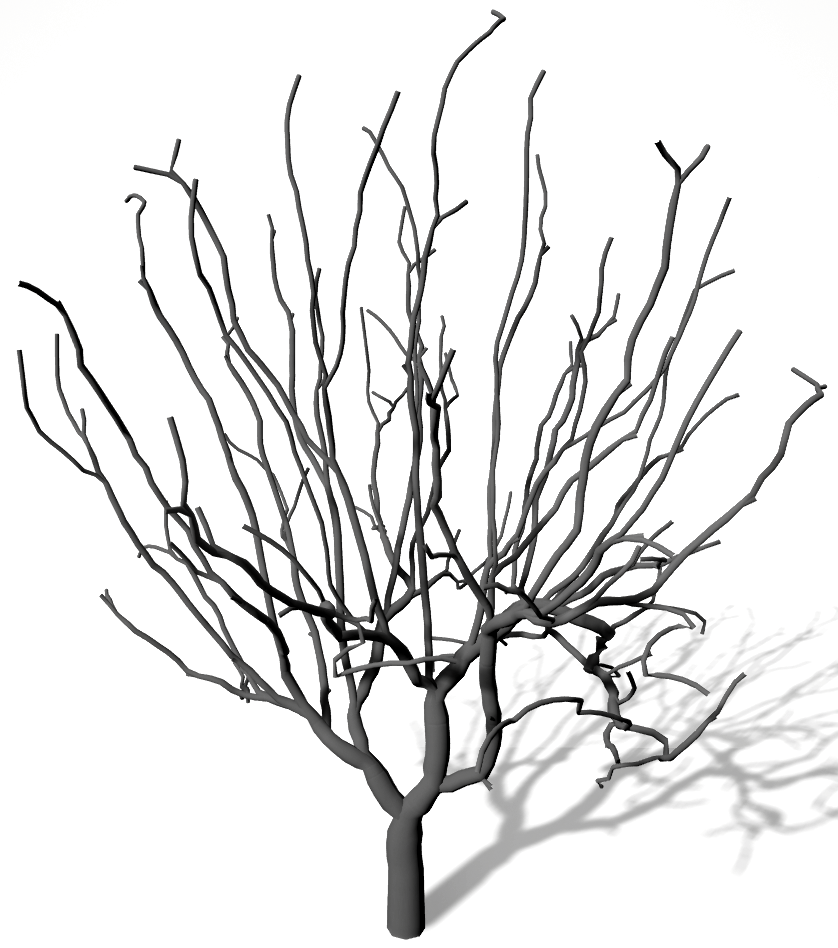
\includegraphics[height=.21\textheight]{images/SCA_SI_Iterationen80.png}
		\caption{$N_I = 80$}
		\label{subfig:SCA_SI_Iterationen80}
	\end{subfigure}
	\caption{Wirkung von Schrittweite $D$ und maximaler Anzahl von Iterationen $N_I$ auf die generierte Baumstruktur. Eigene Abbildungen.}
	\label{fig:SCA_SI}
\end{figure}


\paragraph{Gewichtetes Wachstum}

Gewichtetes Wachstum erhöht die Wachstums-Schrittweite der Astsegmente in Abhängigkeit von der Zweigtiefe. Dies führt zu der erkennbaren Bildung eines Stammes und den davon abzweigenden Hauptästen. 

Die Einstellung erzielt den besten visuellen Eindruck in bestimmten Situationen: Bei Anwendung des Algorithmus auf große Werte für den Radius des Einflussbereichs $r$, der Anzahl von Einflusspunkten $N$, dem Einflussradius $d_i$ und bei einer Begrenzung des maximalen Anzahl durchzuführender Iterationen $N_I$, sodass die Baumstruktur nur einen Teil des Einflussbereichs ausfüllen kann. Dies erweckt den Anschein eines Baumes, dessen Wachstum noch nicht beendet ist.

Abbildung \ref{fig:SCA_GewWachstum} zeigt ein Beispiel für die Anwendung von gewichtetem Wachstum in der beschriebenen Situation.

\begin{figure} [hbtp]
	\centering
	\begin{subfigure}[t]{.45\textwidth}
		\centering
		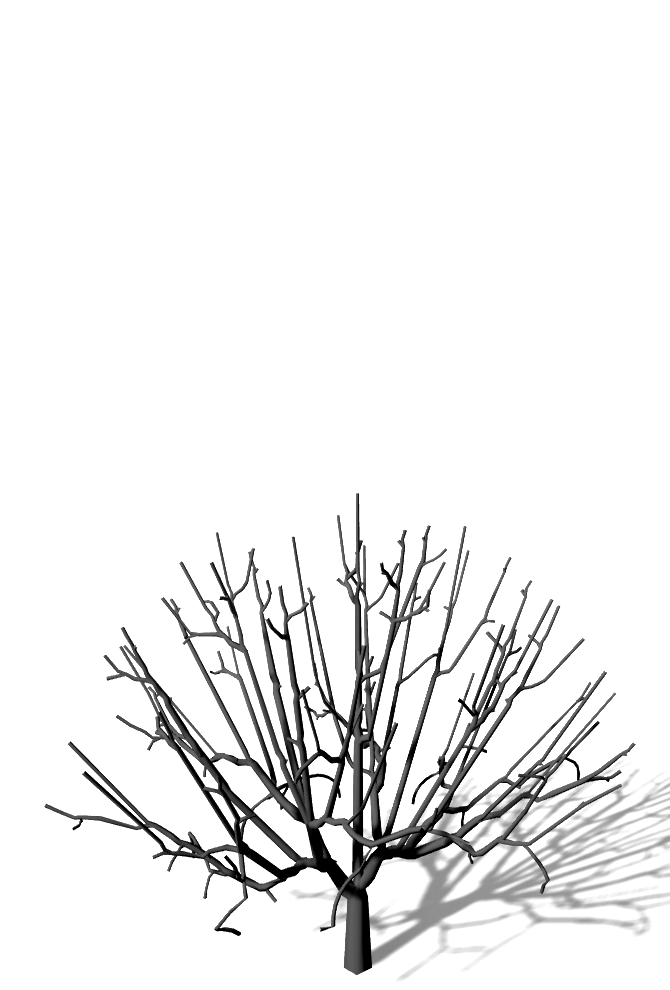
\includegraphics[height=.3\textheight]{images/SCA_GewWachstum_Off.png}
		\caption{$N = 5000$, $r = 1000$, $N_I = 50$, $d_k = 50$, $d_i = 1000$, $D = 15$, $\protect\overrightarrow{T} = (0,0,0.7)$, kein gewichtetes Wachstum.}
		\label{subfig:SCA_GewWachstum_Off}
	\end{subfigure}
	\hspace{.05\linewidth}
	\begin{subfigure}[t]{.45\textwidth}
		\centering
		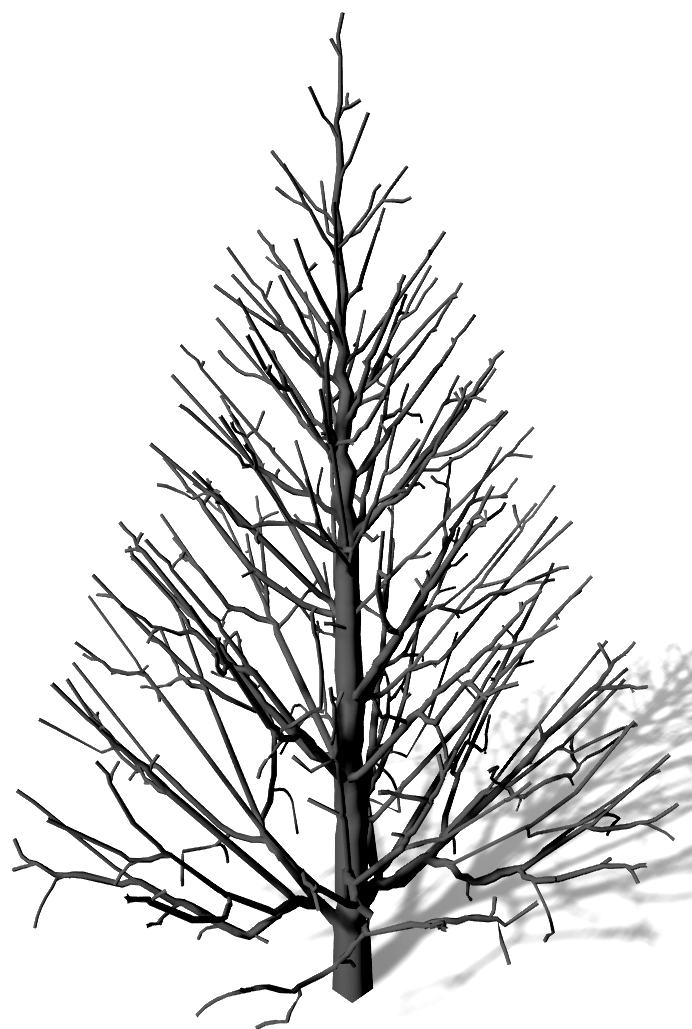
\includegraphics[height=.3\textheight]{images/SCA_GewWachstum_On.png}
		\caption{Mit gewichtetem Wachstum.}
		\label{subfig:SCA_GewWachstum_On}
	\end{subfigure}	
	\caption{Wirkung von gewichtetem Wachstum auf die generierte Baumstruktur. Eigene Abbildungen.}
	\label{fig:SCA_GewWachstum}
\end{figure}


\section{Effizienz}

Die Effizienz einer Software ist ihre Fähigkeit, mit den durch das Betriebssystem bereitgestellten Ressourcen ein bestimmtes Leistungsniveau zu erzielen. \cite[S.259]{Softwaremanagement:98} In Hinsicht auf prozedurale Generierung muss auf zwei wesentliche Punkte geachtet werden: Die Generierungszeit und das Laufzeitverhalten.

\subsection{Generierungszeit}

Die Zeit welche benötigt wird um eine Baumstruktur aufzubauen wird als Generierungszeit bezeichnet und bei den Implementierungen durch die übergebenen Parameter beeinflusst. Mithilfe des Unreal Engine Profilers wurde die Ausführungszeit bestimmter Funktionen oder Funktionsabschnitte gemessen um die Abhängigkeiten zwischen Parametern und Generierungszeit zu bestimmen. \cite{Profiling:15}

\paragraph{L-System-Actor}

Die Generierungszeit der L-System Implementierung hängt linear von den durch die Turtle-Interpretation ausgeführten Bewegungen und Rotationen ab und macht diese somit abhängig von der Anzahl der Ableitungen sowie den angegebenen Produktionsregeln. Je öfter ein Axiom abgeleitet wird und je mehr Rotations- und Bewegungsaktionen in den Nachfolgern der Produktionsregeln angegeben sind, desto mehr Aktionen enthält die zu interpretierende Zeichenkette. 

\paragraph{Space-Colonization-Actor}

Die Generierungszeit der Space-Colonization Implementierung wird durch eine Vielzahl von Parametern festgelegt, welche die Anzahl der Einflusspunkte, wachsenden Astsegmente und durchzuführenden Iterationen beeinflussen. In einer Iteration wird jeder Einflusspunkt daraufhin überprüft, ob sich mindestens einer der wachsenden Astsegmente in seinem Einflussradius befindet. Falls dies zutrifft wird zusätzlich die Liste der Astsegmente im Einflussradius daraufhin überprüft, welches Segment den geringsten Abstand besitzt.

Die eingeführte Bedingung $max_{NG}$ -- die maximale Anzahl von Iterationen, in welchen einem Astsegment kein neuer Nachfolger hinzugefügt wurde -- begrenzt die Anzahl der aktuell wachsenden Astsegmente und konnte somit erfolgreich zur Verringerung der Generierungszeit eingesetzt werden, ohne die resultierende Baumstruktur visuell erkennbar zu verändern. 

Abbildung \ref{fig:SCA_maxNG} zeigt zwei mit denselben Parametern generierte Space-Colo\-ni\-za\-tion Baumstrukturen, lediglich $max_{NG}$ wurde angepasst. Die Generierungszeit der Baumstruktur aus Abbildung \ref{subfig:SCA_maxNG1000} beträgt ungefähr das fünffache der Generierungszeit des Modells aus Abbildung \ref{subfig:SCA_maxNG2}. Die Messung der Generierungszeit fand unter gleichbleibenden Bedingungen auf einem Rechner mit $3.3GHz$ Prozessor statt. 

\begin{figure} [hbtp]
	\centering
	\begin{subfigure}[t]{.45\textwidth}
		\centering
		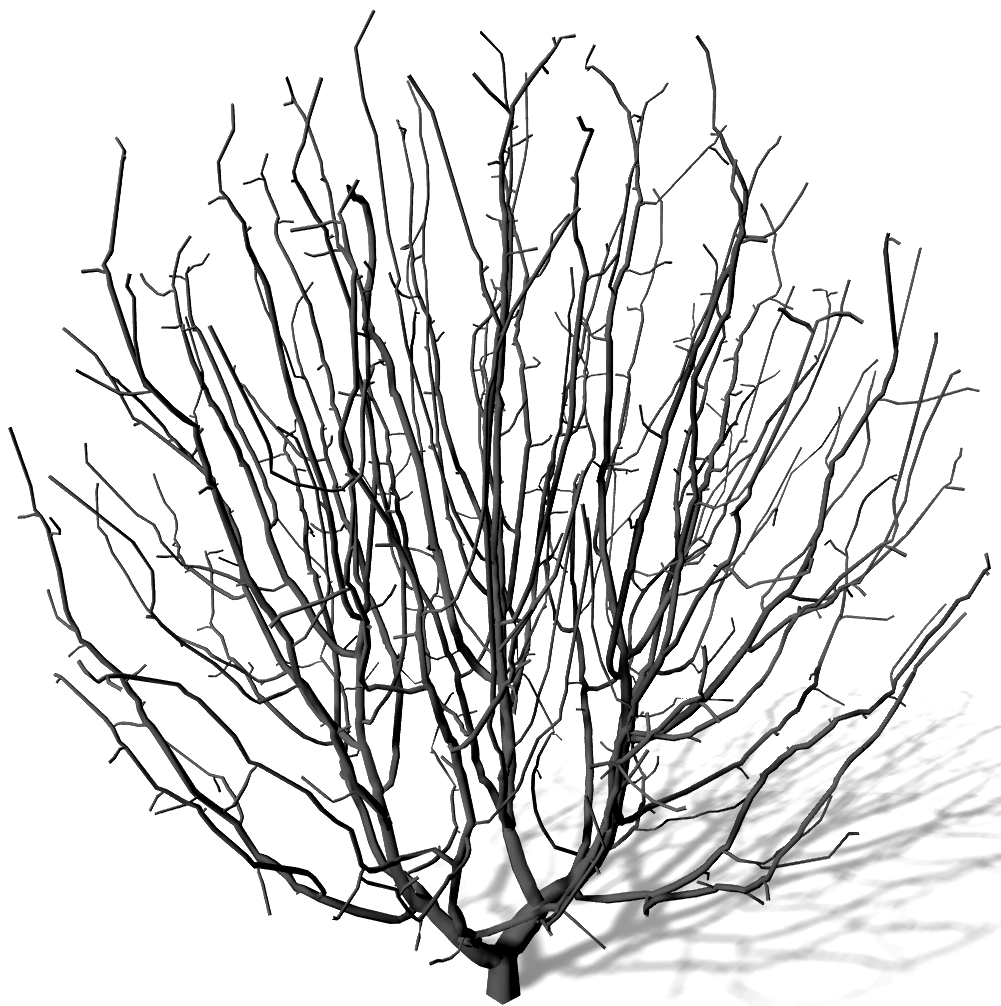
\includegraphics[height=.2\textheight]{images/SCA_maxNG_2.png}
		\caption{$N = 5000$, $r = 1000$, $N_I = 1000$, $d_k = 100$, $d_i = 250$, $D = 20$, $\protect\overrightarrow{T} = (0,0,0.2)$. \\ $max_{NG} = 2$, $Generierungszeit = 1.12 s$.}
		\label{subfig:SCA_maxNG2}
	\end{subfigure}
	\hspace{.05\linewidth}
	\begin{subfigure}[t]{.45\textwidth}
		\centering
		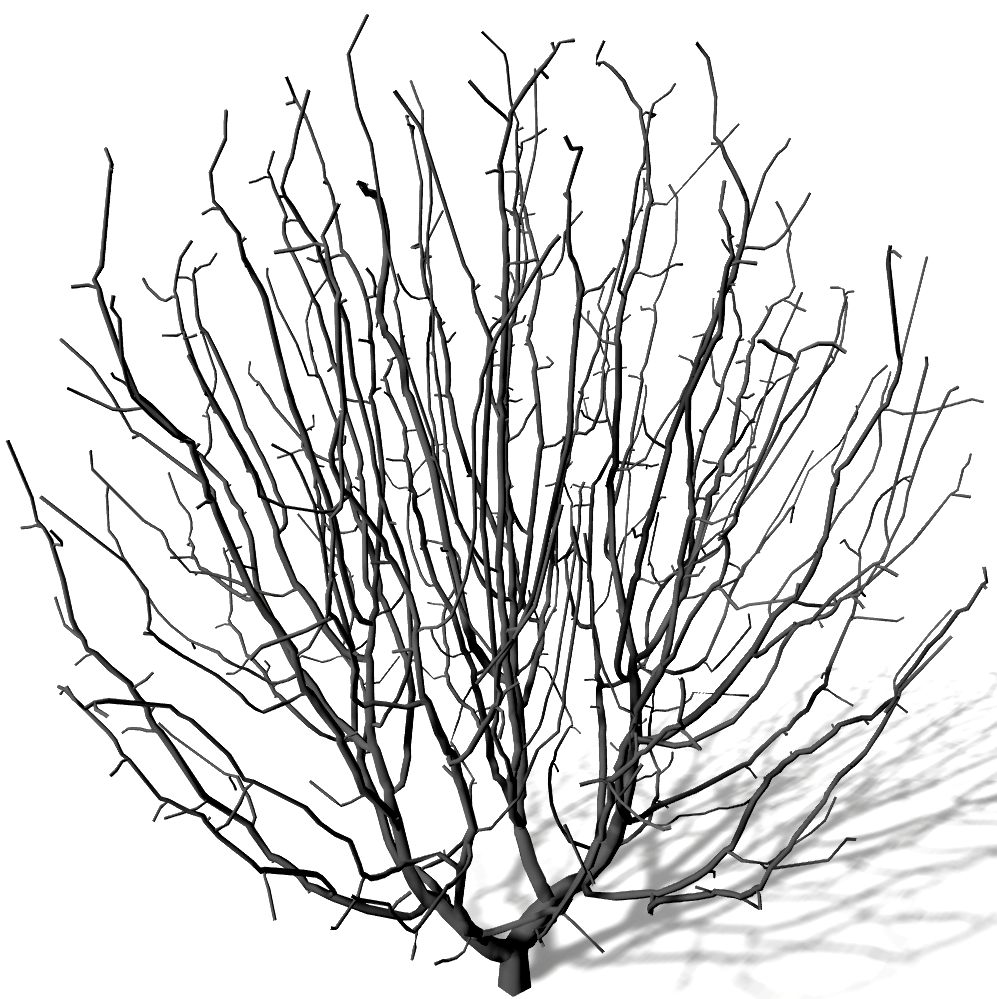
\includegraphics[height=.2\textheight]{images/SCA_maxNG_1000.png}
		\caption{$max_{NG} = 1000$, $Generierungszeit = 6.08 s$.}
		\label{subfig:SCA_maxNG1000}
	\end{subfigure}	
	\caption{Einfluss von $max_{NG}$ auf die Generierungszeit. Die Messungen der Generierungszeit fanden unter gleichbleibenden Bedingungen statt. Eigene Abbildungen.}
	\label{fig:SCA_maxNG}
\end{figure}

\subsection{Laufzeitverhalten}

Das Laufzeitverhalten entspricht in diesem Fall der Anzahl von Bildern (engl.: Frames), die pro Sekunde produziert werden können, auch als Bildrate (engl.: Frames per second oder fps) bezeichnet. In Hinsicht auf die generierten Baumstrukturen ist das Laufzeitverhalten abhängig von der dargestellten Geometrie, da eine Grafikkarte lediglich eine begrenzte Menge Vertexdaten pro Sekunde verarbeiten und darstellen kann. Eine Verbesserung des Laufzeitverhaltens wird durch eine Reduktion der Vertexmenge einer generierten Baumstruktur erreicht.

Das Laufzeitverhalten muss stets gegen die Qualität der zu generierenden Modelle abgewägt werden -- eine Verringerung der Vertexdaten führt zwar zu einer höheren Bildrate, im Gegenzug jedoch auch zu einer niedrigeren visuellen Modellqualität. \cite[S.5]{Deussen:05}

\paragraph{L-System-Actor}

Die Vertexanzahl eines durch ein L-System generierten Baummodells wird durch die Anzahl der Schritte bestimmt, welche von der Turtle-Interpretation durchgeführt werden und ist somit abhängig von der Anzahl an Ableitungen und den definierten Produktionsregeln. 

\paragraph{Space-Colonization-Actor}

Die Anzahl von Vertizes, welche durch die Space-Colonization Implementierung generiert werden, hängt von Parametern ab, welche die Anzahl der erstellen Astsegmente beeinflussen. Insbesondere eine Verringerung der Schrittweite und des Minimalradius tragen zu einer Erhöhung der Anzahl an generierten Astsegmenten bei.

\paragraph{Modellgenerierungssystem}

Das Modellgenerierungssystem bietet drei Parameter zur Anpassung der Modellqualität: die minimale und maximale Anzahl von Zylindersektionen sowie den Kurvenreduktionswert, welche sich auf generierte Bäume beider Implementierungen anwenden lassen.

Für jedes Astsegment wird die Anzahl an Zylindersektionen festgelegt, indem, abhängig von der Zweigtiefe des Segments, zwischen der minimalen und maximalen Anzahl $n_{min}$ und $n_{max}$ linear interpoliert wird. Das Resultat ist, dass Astsegmente mit einer hohen Zweigtiefe und geringem Radius mit weniger Vertizes dargestellt werden als Astsegmente mit einer niedrigen Zweigtiefe und großem Radius.

Der Kurvenreduktionswert $max_K$ reduziert die Zahl der Astsegmente, indem Segmente, die in einem geringen Winkel voneinander abstehen, zusammen gefasst werden. Die geringere Astsegmentanzahl führt zu einer Verringerung der Vertexanzahl.

\begin{figure} [hbtp]
	\centering
	\begin{subfigure}[t]{.45\textwidth}
		\centering
		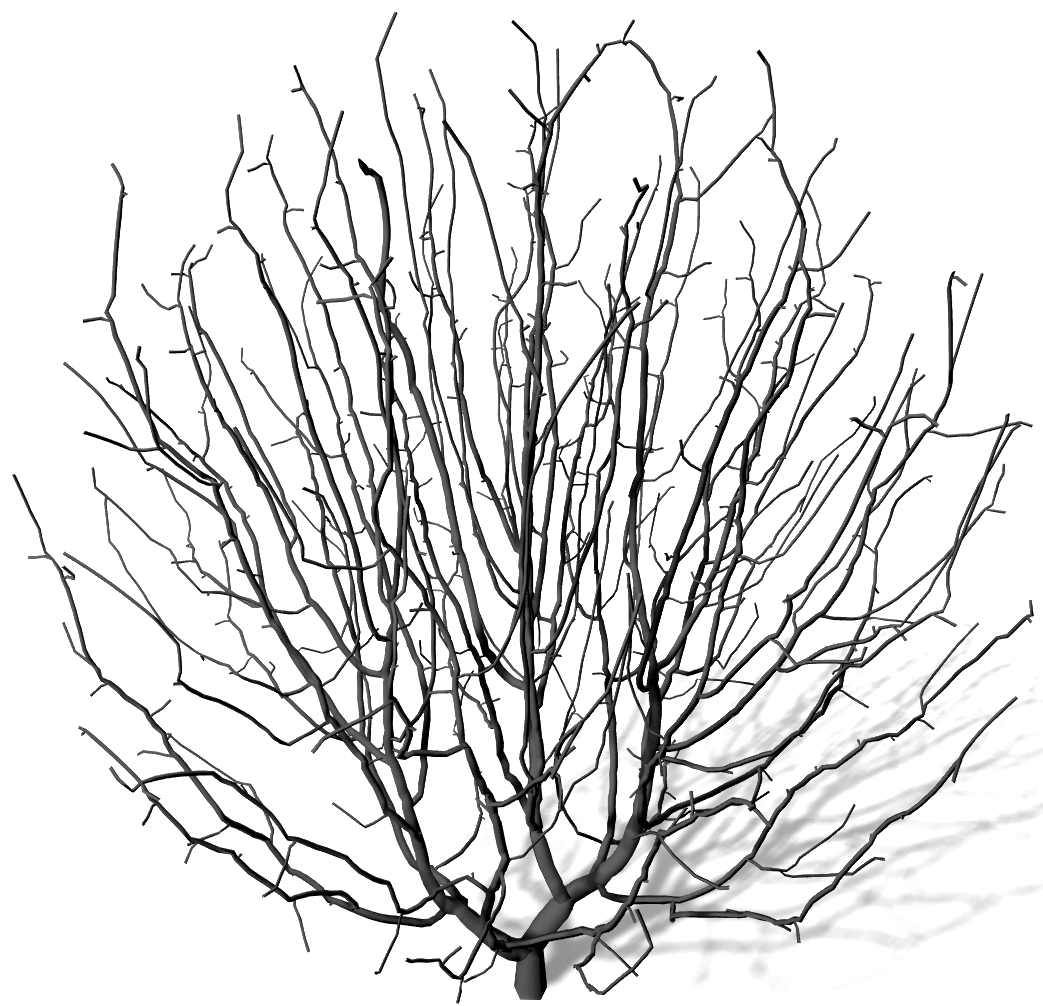
\includegraphics[height=.2\textheight]{images/SCA_Quali_SegmentsLow.png}
		\caption{$n_{min} = 3$, $n_{max} = 5$, $max_K = 1.0$\\ $N_V = 23565$.}
		\label{subfig:SCA_Quali_SegmentsLow}
	\end{subfigure}
	\hspace{.05\linewidth}
	\begin{subfigure}[t]{.45\textwidth}
		\centering
		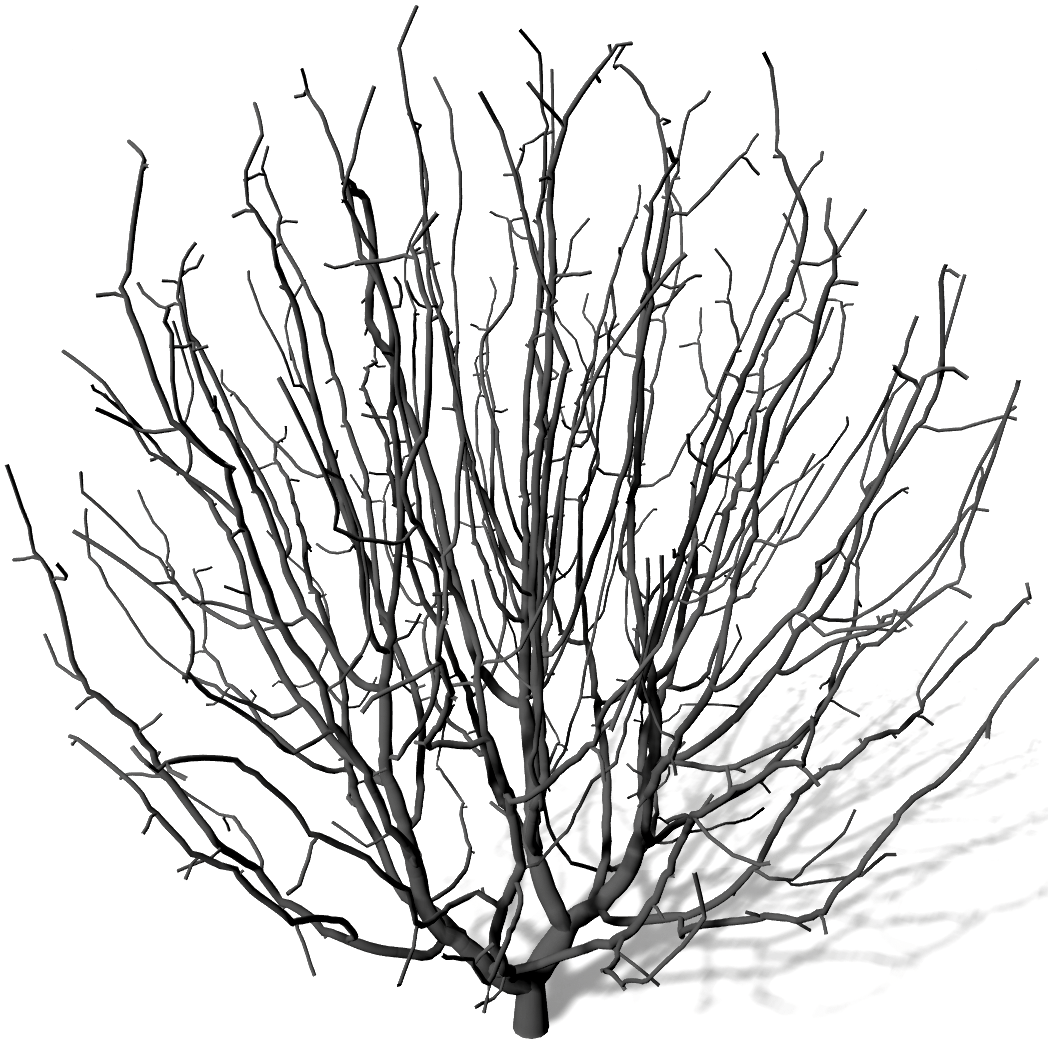
\includegraphics[height=.2\textheight]{images/SCA_Quali_SegmentsHigh.png}
		\caption{$n_{min} = 8$, $n_{max} = 12$, $max_K = 1.0$\\ $N_V = 54009$.}
		\label{subfig:SCA_Quali_SegmentsHigh}
	\end{subfigure}	
	\begin{subfigure}[t]{.45\textwidth}
		\centering
		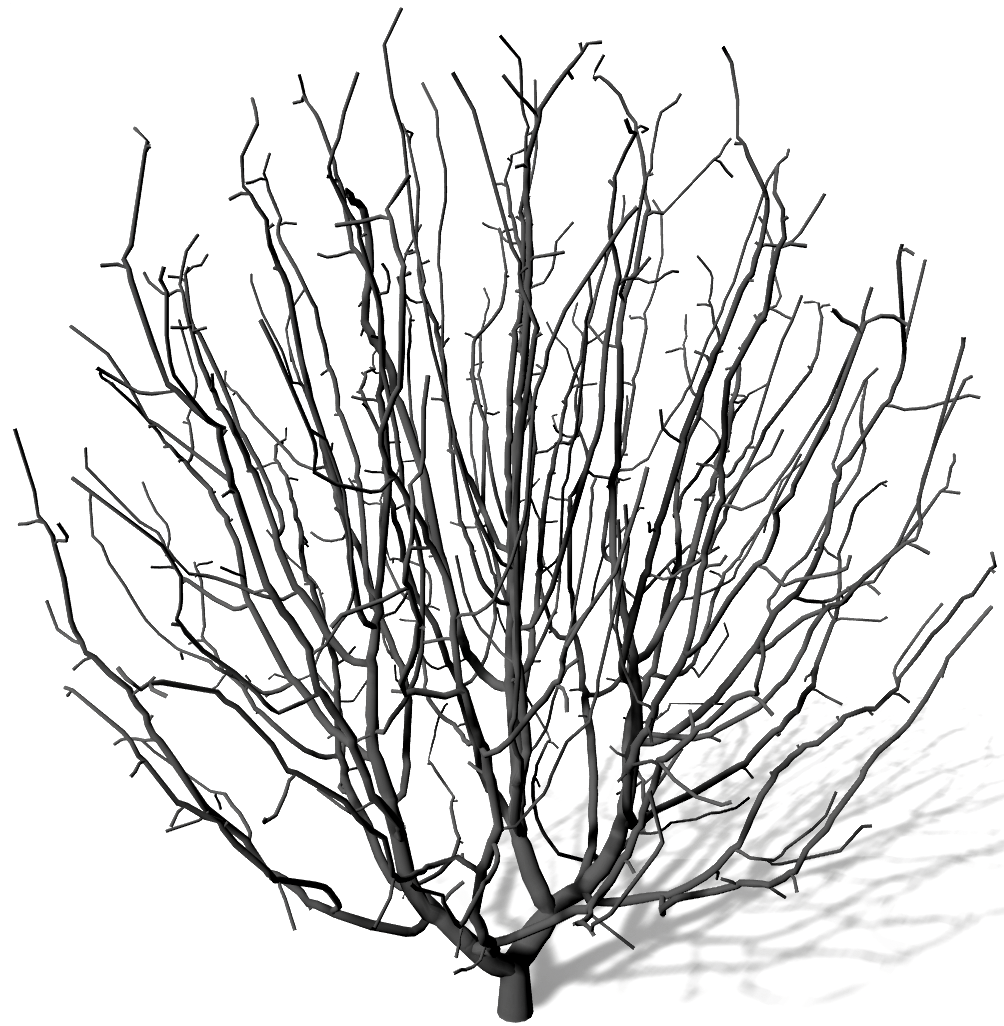
\includegraphics[height=.2\textheight]{images/SCA_Quali_CR_Low.png}
		\caption{$n_{min} = 8$, $n_{max} = 12$, $max_K = 0.99$\\ $N_V = 34709$.}
		\label{subfig:SCA_Quali_CR_Low}
	\end{subfigure}
	\hspace{.05\linewidth}
	\begin{subfigure}[t]{.45\textwidth}
		\centering
		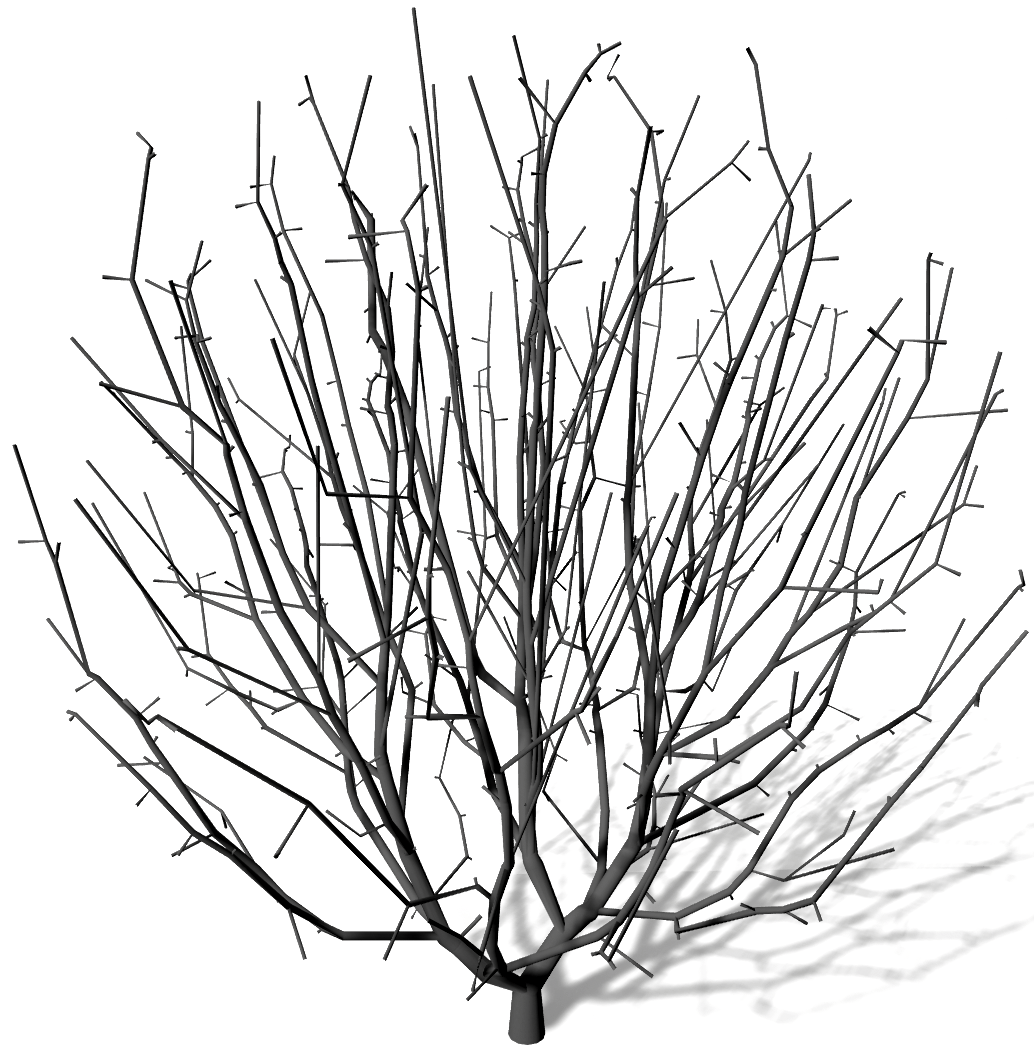
\includegraphics[height=.2\textheight]{images/SCA_Quali_CR_High.png}
		\caption{$n_{min} = 8$, $n_{max} = 12$, $max_K = 0.5$\\ $N_V = 14130$.}
		\label{subfig:SCA_Quali_CR_High}
	\end{subfigure}	
	\caption{Einfluss der minimalen und maximalen Anzahl an Zylindersektionen $n_{min}$ und $n_{max}$ sowie des Kurvenreduktionswerts $max_K$ auf die Zahl der generierten Vertizes $N_V$. Die Parameter für die Generierung des zugrunde liegenden graphentheoretischen Baums stimmen überein. Eigene Abbildungen.}
	\label{fig:SCA_Quali}
\end{figure}


